% !TeX spellcheck = hu_HU
% !TeX encoding = UTF-8
% !TeX program = xelatex
%TODO Change language to en_GB (recommended) or en_US for English documents
\documentclass[12pt,a4paper,oneside, lmargin=3.5cm, rmargin=2.5cm]{report}             % Single-side
%\documentclass[11pt,a4paper,twoside,openright]{report}  % Duplex

% thanks to http://tex.stackexchange.com/a/47579/71109
\usepackage{ifxetex}
\usepackage{ifluatex}
\newif\ifxetexorluatex % a new conditional starts as false
\ifnum 0\ifxetex 1\fi\ifluatex 1\fi>0
   \xetexorluatextrue
\fi

\ifxetexorluatex
  \usepackage{fontspec}
\else
  \usepackage[T1]{fontenc}
  \usepackage[utf8]{inputenc}
  \usepackage[lighttt]{lmodern}
\fi

\usepackage[english,magyar]{babel} % Alapértelmezés szerint utoljára definiált nyelv lesz aktív, de később külön beállítjuk az aktív nyelvet.

%\usepackage{cmap}
\usepackage{amsfonts,amsmath,amssymb} % Mathematical symbols.
%\usepackage[ruled,boxed,resetcount,linesnumbered]{algorithm2e} % For pseudocodes. % beware: this is not compatible with LuaLaTeX, see http://tex.stackexchange.com/questions/34814/lualatex-and-algorithm2e
\usepackage{booktabs} % For publication quality tables for LaTeX
\usepackage{graphicx}

%\usepackage{fancyhdr}
%\usepackage{lastpage}

\usepackage{anysize}
%\usepackage{sectsty}
\usepackage{setspace} % For setting line spacing

\usepackage[unicode]{hyperref} % For hyperlinks in the generated document.
\usepackage{xcolor}
\usepackage{listings} % For source code snippets.

\usepackage[amsmath,thmmarks]{ntheorem} % Theorem-like environments.

\usepackage[hang]{caption}

\singlespacing

\newcommand{\selecthungarian}{
	\selectlanguage{magyar}
	\setlength{\parindent}{2em}
	\setlength{\parskip}{0em}
	\frenchspacing
}

\newcommand{\selectenglish}{
	\selectlanguage{english}
	\setlength{\parindent}{0em}
	\setlength{\parskip}{0.5em}
	\nonfrenchspacing
	\renewcommand{\figureautorefname}{Figure}
	\renewcommand{\tableautorefname}{Table}
	\renewcommand{\partautorefname}{Part}
	\renewcommand{\chapterautorefname}{Chapter}
	\renewcommand{\sectionautorefname}{Section}
	\renewcommand{\subsectionautorefname}{Section}
	\renewcommand{\subsubsectionautorefname}{Section}
}

\usepackage[numbers]{natbib}
\usepackage{xspace}
\usepackage{pdfpages}
\usepackage{url}
\def\UrlBreaks{\do\/\do-}

%TODO Set the main variables
\newcommand{\vikszerzoVezeteknev}{Dobsinszki}
\newcommand{\vikszerzoKeresztnev}{Gergely}

\newcommand{\vikkonzulensAMegszolitas}{dr.~}
\newcommand{\vikkonzulensAVezeteknev}{Mihajlik}
\newcommand{\vikkonzulensAKeresztnev}{Péter}

\newcommand{\vikkonzulensBMegszolitas}{}
\newcommand{\vikkonzulensBVezeteknev}{}
\newcommand{\vikkonzulensBKeresztnev}{}

\newcommand{\vikkonzulensCMegszolitas}{}
\newcommand{\vikkonzulensCVezeteknev}{}
\newcommand{\vikkonzulensCKeresztnev}{}

\newcommand{\vikcim}{Mély neuronháló alapú orosz nyelvű beszédfelismerő fejlesztése} % Cím
\newcommand{\viktanszek}{\bmetmit} % Tanszék
\newcommand{\vikdoktipus}{\bsc} % Dokumentum típusa (\bsc vagy \msc)
\newcommand{\vikmunkatipusat}{szakdolgozatot} % a "hallgató nyilatkozat" részhez: szakdolgozatot vagy diplomatervet

%--------------------------------------------------------------------------------------
% TDK-specifikus változók
%--------------------------------------------------------------------------------------
\newcommand{\tdkszerzoB}{Második Szerző} % Második szerző neve; hagyd üresen, ha egyedül írtad a TDK-t.
\newcommand{\tdkev}{2014} % A dolgozat írásának éve (pl. "2014") (Ez OTDK-nál eltérhet az aktuális évtől.)

% További adatok az OTDK címlaphoz (BME-s TDK-hoz nem kell kitölteni)
\newcommand{\tdkevfolyamA}{IV} % Első szerző évfolyama, római számmal (pl. IV).
\newcommand{\tdkevfolyamB}{III} % Második szerző évfolyama, római számmal (pl. III).
\newcommand{\tdkkonzulensbeosztasA}{egyetemi tanár} % Első konzulens beosztása (pl. egyetemi docens)
\newcommand{\tdkkonzulensbeosztasB}{doktorandusz} % Második konzulens beosztása (pl. egyetemi docens)

\newcommand{\szerzoMeta}{\vikszerzoVezeteknev{} \vikszerzoKeresztnev} % egy szerző esetén
%\newcommand{\szerzoMeta}{\vikszerzoVezeteknev{} \vikszerzoKeresztnev, \tdkszerzoB} % két szerző esetén

%TODO Language configuration -- choose one
% Beállítások magyar nyelvű dolgozathoz
%--------------------------------------------------------------------------------------
% Elnevezések
%--------------------------------------------------------------------------------------
\newcommand{\bme}{Budapesti Műszaki és Gazdaságtudományi Egyetem}
\newcommand{\vik}{Villamosmérnöki és Informatikai Kar}

\newcommand{\bmemit}{Méréstechnika és Információs Rendszerek Tanszék}
\newcommand{\bmetmit}{Távközlési és Médiainformatikai Tanszék}

\newcommand{\keszitette}{Készítette}
\newcommand{\konzulens}{Konzulens}

\newcommand{\bsc}{Szakdolgozat}
\newcommand{\msc}{Diplomaterv}
\newcommand{\tdk}{TDK dolgozat}
\newcommand{\bsconlab}{BSc Önálló laboratórium}
\newcommand{\msconlabi}{MSc Önálló laboratórium 1.}
\newcommand{\msconlabii}{MSc Önálló laboratórium 2.}

\newcommand{\pelda}{Példa}
\newcommand{\definicio}{Definíció}
\newcommand{\tetel}{Tétel}

\newcommand{\bevezetes}{Bevezetés}
\newcommand{\koszonetnyilvanitas}{Köszönetnyilvánítás}
\newcommand{\fuggelek}{Függelék}

% Opcionálisan átnevezhető címek
%\addto\captionsmagyar{%
%\renewcommand{\listfigurename}{Saját ábrajegyzék cím}
%\renewcommand{\listtablename}{Saját táblázatjegyzék cím}
%\renewcommand{\bibname}{Saját irodalomjegyzék név}
%}

\newcommand{\szerzo}{\vikszerzoVezeteknev{} \vikszerzoKeresztnev}
\newcommand{\vikkonzulensA}{\vikkonzulensAMegszolitas\vikkonzulensAVezeteknev{} \vikkonzulensAKeresztnev}
\newcommand{\vikkonzulensB}{\vikkonzulensBMegszolitas\vikkonzulensBVezeteknev{} \vikkonzulensBKeresztnev}
\newcommand{\vikkonzulensC}{\vikkonzulensCMegszolitas\vikkonzulensCVezeteknev{} \vikkonzulensCKeresztnev}

\newcommand{\selectthesislanguage}{\selecthungarian}

\bibliographystyle{huplain}

\def\lstlistingname{lista}

\newcommand{\appendixnumber}{6}  % a fofejezet-szamlalo az angol ABC 6. betuje (F) lesz

% Settings for English documents
%%--------------------------------------------------------------------------------------
% Elnevezések
%--------------------------------------------------------------------------------------
\newcommand{\bme}{Budapest University of Technology and Economics}
\newcommand{\vik}{Faculty of Electrical Engineering and Informatics}

\newcommand{\bmemit}{Department of Measurement and Information Systems}

\newcommand{\keszitette}{Author}
\newcommand{\konzulens}{Advisor}

\newcommand{\bsc}{Bachelor's Thesis}
\newcommand{\msc}{Master's Thesis}
\newcommand{\tdk}{Scientific Students' Association Report}
\newcommand{\bsconlab}{BSc Project Laboratory}
\newcommand{\msconlabi}{MSc Project Laboratory 1}
\newcommand{\msconlabii}{MSc Project Laboratory 2}

\newcommand{\pelda}{Example}
\newcommand{\definicio}{Definition}
\newcommand{\tetel}{Theorem}

\newcommand{\bevezetes}{Introduction}
\newcommand{\koszonetnyilvanitas}{Acknowledgements}
\newcommand{\fuggelek}{Appendix}

% Optional custom titles
%\addto\captionsenglish{%
%\renewcommand*{\listfigurename}{Your list of figures title}
%\renewcommand*{\listtablename}{Your list of tables title}
%\renewcommand*{\bibname}{Your bibliography title}
%}

\newcommand{\szerzo}{\vikszerzoKeresztnev{} \vikszerzoVezeteknev}
\newcommand{\vikkonzulensA}{\vikkonzulensAMegszolitas\vikkonzulensAKeresztnev{} \vikkonzulensAVezeteknev}
\newcommand{\vikkonzulensB}{\vikkonzulensBMegszolitas\vikkonzulensBKeresztnev{} \vikkonzulensBVezeteknev}
\newcommand{\vikkonzulensC}{\vikkonzulensCMegszolitas\vikkonzulensCKeresztnev{} \vikkonzulensCVezeteknev}

\newcommand{\selectthesislanguage}{\selectenglish}

\bibliographystyle{plainnat}

\newcommand{\ie}{i.e.\@\xspace}
\newcommand{\Ie}{I.e.\@\xspace}
\newcommand{\eg}{e.g.\@\xspace}
\newcommand{\Eg}{E.g.\@\xspace}
\newcommand{\etal}{et al.\@\xspace}
\newcommand{\etc}{etc.\@\xspace}
\newcommand{\vs}{vs.\@\xspace}
\newcommand{\viz}{viz.\@\xspace} % videlicet
\newcommand{\cf}{cf.\@\xspace} % confer
\newcommand{\Cf}{Cf.\@\xspace}
\newcommand{\wrt}{w.r.t.\@\xspace} % with respect to
\newcommand{\approximately}{approx.\@\xspace}

\newcommand{\appendixnumber}{1}  % a fofejezet-szamlalo az angol ABC 1. betuje (A) lesz


%--------------------------------------------------------------------------------------
% Page layout setup
%--------------------------------------------------------------------------------------
% we need to redefine the pagestyle plain
% another possibility is to use the body of this command without \fancypagestyle
% and use \pagestyle{fancy} but in that case the special pages
% (like the ToC, the References, and the Chapter pages)remain in plane style

\pagestyle{plain}
\marginsize{35mm}{25mm}{15mm}{15mm}

\setcounter{tocdepth}{3}
%\sectionfont{\large\upshape\bfseries}
\setcounter{secnumdepth}{3}

\sloppy % Margón túllógó sorok tiltása.
\widowpenalty=10000 \clubpenalty=10000 %A fattyú- és árvasorok elkerülése
\def\hyph{-\penalty0\hskip0pt\relax} % Kötőjeles szavak elválasztásának engedélyezése


%--------------------------------------------------------------------------------------
% Setup hyperref package
%--------------------------------------------------------------------------------------
\hypersetup{
    % bookmarks=true,            % show bookmarks bar?
    unicode=true,              % non-Latin characters in Acrobat's bookmarks
    pdftitle={\vikcim},        % title
    pdfauthor={\szerzoMeta},    % author
    pdfsubject={\vikdoktipus}, % subject of the document
    pdfcreator={\szerzoMeta},   % creator of the document
    pdfproducer={},    % producer of the document
    pdfkeywords={},    % list of keywords (separate then by comma)
    pdfnewwindow=true,         % links in new window
    colorlinks=true,           % false: boxed links; true: colored links
    linkcolor=black,           % color of internal links
    citecolor=black,           % color of links to bibliography
    filecolor=black,           % color of file links
    urlcolor=black             % color of external links
}


%--------------------------------------------------------------------------------------
% Set up listings
%--------------------------------------------------------------------------------------
\definecolor{lightgray}{rgb}{0.95,0.95,0.95}
\lstset{
	basicstyle=\scriptsize\ttfamily, % print whole listing small
	keywordstyle=\color{black}\bfseries, % bold black keywords
	identifierstyle=, % nothing happens
	% default behavior: comments in italic, to change use
	% commentstyle=\color{green}, % for e.g. green comments
	stringstyle=\scriptsize,
	showstringspaces=false, % no special string spaces
	aboveskip=3pt,
	belowskip=3pt,
	backgroundcolor=\color{lightgray},
	columns=flexible,
	keepspaces=true,
	escapeinside={(*@}{@*)},
	captionpos=b,
	breaklines=true,
	frame=single,
	float=!ht,
	tabsize=2,
	literate=*
		{á}{{\'a}}1	{é}{{\'e}}1	{í}{{\'i}}1	{ó}{{\'o}}1	{ö}{{\"o}}1	{ő}{{\H{o}}}1	{ú}{{\'u}}1	{ü}{{\"u}}1	{ű}{{\H{u}}}1
		{Á}{{\'A}}1	{É}{{\'E}}1	{Í}{{\'I}}1	{Ó}{{\'O}}1	{Ö}{{\"O}}1	{Ő}{{\H{O}}}1	{Ú}{{\'U}}1	{Ü}{{\"U}}1	{Ű}{{\H{U}}}1
}


%--------------------------------------------------------------------------------------
% Set up theorem-like environments
%--------------------------------------------------------------------------------------
% Using ntheorem package -- see http://www.math.washington.edu/tex-archive/macros/latex/contrib/ntheorem/ntheorem.pdf

\theoremstyle{plain}
\theoremseparator{.}
\newtheorem{example}{\pelda}

\theoremseparator{.}
%\theoremprework{\bigskip\hrule\medskip}
%\theorempostwork{\hrule\bigskip}
\theorembodyfont{\upshape}
\theoremsymbol{{\large \ensuremath{\centerdot}}}
\newtheorem{definition}{\definicio}

\theoremseparator{.}
%\theoremprework{\bigskip\hrule\medskip}
%\theorempostwork{\hrule\bigskip}
\newtheorem{theorem}{\tetel}


%--------------------------------------------------------------------------------------
% Some new commands and declarations
%--------------------------------------------------------------------------------------
\newcommand{\code}[1]{{\upshape\ttfamily\scriptsize\indent #1}}
\newcommand{\doi}[1]{DOI: \href{http://dx.doi.org/\detokenize{#1}}{\raggedright{\texttt{\detokenize{#1}}}}} % A hivatkozások közt így könnyebb DOI-t megadni.

\DeclareMathOperator*{\argmax}{arg\,max}
%\DeclareMathOperator*[1]{\floor}{arg\,max}
\DeclareMathOperator{\sign}{sgn}
\DeclareMathOperator{\rot}{rot}


%--------------------------------------------------------------------------------------
% Setup captions
%--------------------------------------------------------------------------------------
\captionsetup[figure]{
	width=.75\textwidth,
	aboveskip=10pt}

\renewcommand{\captionlabelfont}{\bf}
%\renewcommand{\captionfont}{\footnotesize\it}

%--------------------------------------------------------------------------------------
% Hyphenation exceptions
%--------------------------------------------------------------------------------------
\hyphenation{Shakes-peare Mar-seilles ár-víz-tű-rő tü-kör-fú-ró-gép}


\author{\vikszerzo}
\title{\viktitle}

%--------------------------------------------------------------------------------------
% Table of contents and the main text
%--------------------------------------------------------------------------------------
\begin{document}

\linespread{1.5}
\pagenumbering{gobble}

%TODO These includes define guidelines -- remove these
%~~~~~~~~~~~~~~~~~~~~~~~~~~~~~~~~~~~~~~~~~~~~~~~~~~~~~~~~~~~~~~~~~~~~~~~~~~~~~~~~~~~~~~
% \selecthungarian
%--------------------------------------------------------------------------------------
% Rovid formai es tartalmi tajekoztato
%--------------------------------------------------------------------------------------

\footnotesize
\begin{center}
\large
\textbf{\Large Általános információk, a diplomaterv szerkezete}\\
\end{center}

A diplomaterv szerkezete a BME Villamosmérnöki és Informatikai Karán:
\begin{enumerate}
\item	Diplomaterv feladatkiírás
\item	Címoldal
\item	Tartalomjegyzék
\item	A diplomatervező nyilatkozata az önálló munkáról és az elektronikus adatok kezeléséről
\item	Tartalmi összefoglaló magyarul és angolul
\item	Bevezetés: a feladat értelmezése, a tervezés célja, a feladat indokoltsága, a diplomaterv felépítésének rövid összefoglalása
\item	A feladatkiírás pontosítása és részletes elemzése
\item	Előzmények (irodalomkutatás, hasonló alkotások), az ezekből levonható következtetések
\item	A tervezés részletes leírása, a döntési lehetőségek értékelése és a választott megoldások indoklása
\item	A megtervezett műszaki alkotás értékelése, kritikai elemzése, továbbfejlesztési lehetőségek
\item	Esetleges köszönetnyilvánítások
\item	Részletes és pontos irodalomjegyzék
\item	Függelék(ek)
\end{enumerate}

Felhasználható a következő oldaltól kezdődő \LaTeX diplomatervsablon dokumentum tartalma. 

A diplomaterv szabványos méretű A4-es lapokra kerüljön. Az oldalak tükörmargóval készüljenek (mindenhol 2,5~cm, baloldalon 1~cm-es kötéssel). Az alapértelmezett betűkészlet a 12 pontos Times New Roman, másfeles sorközzel, de ettől kismértékben el lehet térni, ill. más betűtípus használata is megengedett.

Minden oldalon -- az első négy szerkezeti elem kivételével -- szerepelnie kell az oldalszámnak.

A fejezeteket decimális beosztással kell ellátni. Az ábrákat a megfelelő helyre be kell illeszteni, fejezetenként decimális számmal és kifejező címmel kell ellátni. A fejezeteket decimális aláosztással számozzuk, maximálisan 3 aláosztás mélységben (pl. 2.3.4.1.). Az ábrákat, táblázatokat és képleteket célszerű fejezetenként külön számozni (pl. 2.4. ábra, 4.2. táblázat vagy képletnél (3.2)). A fejezetcímeket igazítsuk balra, a normál szövegnél viszont használjunk sorkiegyenlítést. Az ábrákat, táblázatokat és a hozzájuk tartozó címet igazítsuk középre. A cím a jelölt rész alatt helyezkedjen el.

A képeket lehetőleg rajzoló programmal készítsék el, az egyenleteket egyenlet-szerkesztő segítségével írják le (A \LaTeX~ehhez kézenfekvő megoldásokat nyújt).

Az irodalomjegyzék szövegközi hivatkozása történhet sorszámozva (ez a preferált megoldás) vagy a Harvard-rendszerben (a szerző és az évszám megadásával). A teljes lista névsor szerinti sorrendben a szöveg végén szerepeljen (sorszámozott irodalmi hivatkozások esetén hivatkozási sorrendben). A szakirodalmi források címeit azonban mindig az eredeti nyelven kell megadni, esetleg zárójelben a fordítással. A listában szereplő valamennyi publikációra hivatkozni kell a szövegben (a \LaTeX-sablon a Bib\TeX~segítségével mindezt automatikusan kezeli). Minden publikáció a szerzők után a következő adatok szerepelnek: folyóirat cikkeknél a pontos cím, a folyóirat címe, évfolyam, szám, oldalszám tól-ig. A folyóiratok címét csak akkor rövidítsük, ha azok nagyon közismertek vagy nagyon hosszúak. Internetes hivatkozások megadásakor fontos, hogy az elérési út előtt megadjuk az oldal tulajdonosát és tartalmát (mivel a link egy idő után akár elérhetetlenné is válhat), valamint az elérés időpontját.

\vspace{5mm}
Fontos:
\begin{itemize}
	\item A szakdolgozatkészítő / diplomatervező nyilatkozata (a jelen sablonban szereplő szövegtartalommal) kötelező előírás, Karunkon ennek hiányában a szakdolgozat/diplomaterv nem bírálható és nem védhető!
	\item Mind a dolgozat, mind a melléklet maximálisan 15~MB méretű lehet!
\end{itemize}

\vspace{5mm}
\begin{center}
Jó munkát, sikeres szakdolgozatkészítést, ill. diplomatervezést kívánunk!
\end{center}

\normalsize
\selectthesislanguage

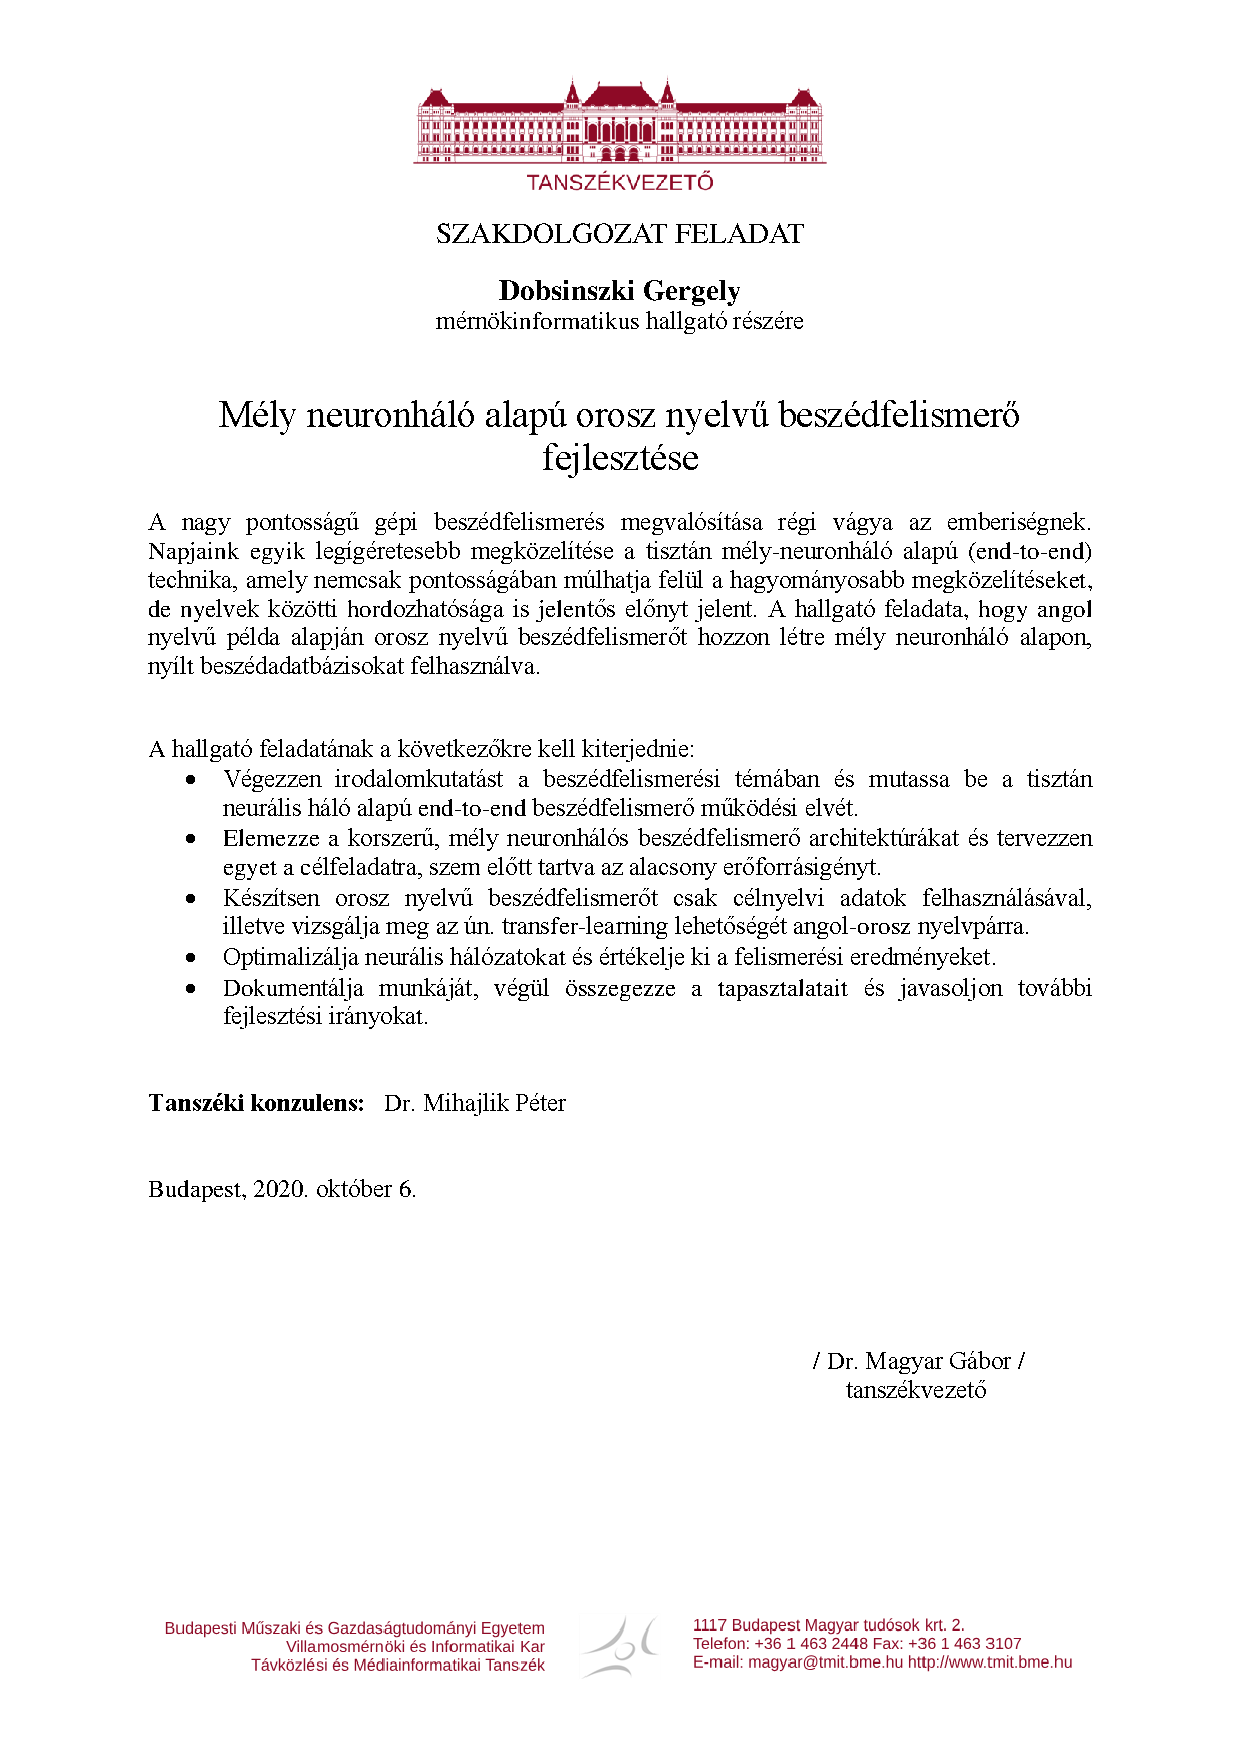
\includepdf[pages=-,pagecommand={}]{feladatkiiras.pdf}
\normalsize
\selectthesislanguage

%TODO Titlepage -- choose one from below
%~~~~~~~~~~~~~~~~~~~~~~~~~~~~~~~~~~~~~~~~~~~~~~~~~~~~~~~~~~~~~~~~~~~~~~~~~~~~~~~~~~~~~~
\hypersetup{pageanchor=false}
%--------------------------------------------------------------------------------------
%	The title page
%--------------------------------------------------------------------------------------
\begin{titlepage}
\begin{center}

\includegraphics[width=60mm,keepaspectratio]{figures/bme_logo.pdf}\\
\vspace{0.3cm}
\textbf{\bme}\\
\textmd{\vik}\\
\textmd{\viktanszek}\\[5cm]

\vspace{0.4cm}
{\huge \bfseries \vikcim}\\[0.8cm]
\vspace{0.5cm}
\textsc{\Large \vikdoktipus}\\[4cm]

{
	\renewcommand{\arraystretch}{0.85}
	\begin{tabular}{cc}
	 \makebox[7cm]{\emph{\keszitette}} & \makebox[7cm]{\emph{\konzulens}} \\ \noalign{\smallskip}
	 \makebox[7cm]{\szerzo} & \makebox[7cm]{\vikkonzulensA} \\
	  & \makebox[7cm]{\vikkonzulensB} \\
	  & \makebox[7cm]{\vikkonzulensC} \\
	\end{tabular}
}

\vfill
{\large \today}
\end{center}
\end{titlepage}
\hypersetup{pageanchor=false}

		   % Szakdolgozat/Diplomaterv címlap
%%% TDK címlap
\begin{titlepage}
  \begin{center}  
  
\includegraphics[width=7cm]{./figures/bme_logo.pdf}
  \vspace{0.3cm}
  
  \bme \\
  \vik \\
  \viktanszek \\
  \vspace{5cm}
  
  \huge {\vikcim}
  \vspace{1.5cm}
  
  \large {\textbf{\tdk}}
  \vfill
    
  {\Large 
  	\keszitette: \\ \vspace{0.3cm}
  	\szerzo \\
	\tdkszerzoB \\
  	\vspace{1.5cm}
  	\konzulens: \\ \vspace{0.3cm}
  	\vikkonzulensA \\
  	\vikkonzulensB \\
  }
  
  \vspace{2cm}
  \large {\tdkev}
 \end{center}
\end{titlepage}
%% Címlap vége
	% TDK címlap
%%% OTDK külső címlap
\begin{titlepage}
  	$\;$ 
	\vspace{5cm}
	
	\begin{center}
	\Huge
	\textbf{TDK-dolgozat}\let\thefootnote\relax\footnote{A dolgozat bemutatását a XXXXXXXXX  ``Lorem ipsum dolor sit amet'' című program támogatta.}
	\end{center}
	
	\vspace{13cm}
	
	\Large
	\hspace{8cm} \szerzo
	
	\hspace{8cm} \tdkszerzoB
	
	\hspace{8cm} \tdkev.
\end{titlepage}

\newpage
\thispagestyle{empty}


%% OTDK belső címlap
\begin{titlepage}
  \begin{center}  
  
\includegraphics[width=7cm]{./figures/bme_logo.pdf}
  \vspace{0.3cm}
  
  \bme \\
  \vik \\
  \viktanszek \\
  \vspace{3.5cm}
  
  \huge {\vikcim}
  \vspace{1.5cm}
  
  \large {\textbf{\vikdoktipus}}
  \vfill
    
  {\Large 
  	{\large \keszitette:} \\ \vspace{0.2cm}
  	\szerzo \\ \tdkevfolyamA. évfolyam \\
	\vspace{0.5cm}
	\tdkszerzoB \\ \tdkevfolyamB. évfolyam \\
  	\vspace{1.5cm}
  	{\large \konzulens:} \\ \vspace{0.2cm}
  	\vikkonzulensA,\\ \tdkkonzulensbeosztasA \\
  	\vspace{0.5cm}
  	\vikkonzulensB,\\ \tdkkonzulensbeosztasB \\
  }
  
  \vspace{2cm}
  \large {\tdkev.}
  
 \end{center}
\end{titlepage}   % OTDK címlap


% Table of Contents
%~~~~~~~~~~~~~~~~~~~~~~~~~~~~~~~~~~~~~~~~~~~~~~~~~~~~~~~~~~~~~~~~~~~~~~~~~~~~~~~~~~~~~~
\tableofcontents\vfill


% Declaration and Abstract
%~~~~~~~~~~~~~~~~~~~~~~~~~~~~~~~~~~~~~~~~~~~~~~~~~~~~~~~~~~~~~~~~~~~~~~~~~~~~~~~~~~~~~~
\selectlanguage{magyar}
\pagenumbering{gobble}
%--------------------------------------------------------------------------------------
% Nyilatkozat
%--------------------------------------------------------------------------------------
\begin{center}
\large
\textbf{HALLGATÓI NYILATKOZAT}\\
\end{center}

Alulírott \emph{\vikszerzoVezeteknev{} \vikszerzoKeresztnev}, szigorló hallgató kijelentem, hogy ezt a \vikmunkatipusat{} meg nem engedett segítség nélkül, saját magam készítettem, csak a megadott forrásokat (szakirodalom, eszközök stb.) használtam fel. Minden olyan részt, melyet szó szerint, vagy azonos értelemben, de átfogalmazva más forrásból átvettem, egyértelműen, a forrás megadásával megjelöltem.

Hozzájárulok, hogy a jelen munkám alapadatait (szerző(k), cím, angol és magyar nyelvű tartalmi kivonat, készítés éve, konzulens(ek) neve) a BME VIK nyilvánosan hozzáférhető elektronikus formában, a munka teljes szövegét pedig az egyetem belső hálózatán keresztül (vagy autentikált felhasználók számára) közzétegye. Kijelentem, hogy a benyújtott munka és annak elektronikus verziója megegyezik. Dékáni engedéllyel titkosított diplomatervek esetén a dolgozat szövege csak 3 év eltelte után válik hozzáférhetővé.

\begin{flushleft}
\vspace*{1cm}
Budapest, \today
\end{flushleft}

\begin{flushright}
 \vspace*{1cm}
 \makebox[7cm]{\rule{6cm}{.4pt}}\\
 \makebox[7cm]{\emph{\vikszerzoVezeteknev{} \vikszerzoKeresztnev}}\\
 \makebox[7cm]{hallgató}
\end{flushright}
\thispagestyle{empty}

\vfill
\clearpage
\thispagestyle{empty} % an empty page

\selectthesislanguage
 %TODO Hallgatói nyilatkozat -- TDK és OTDK esetén törlendő!
\pagenumbering{roman}
\setcounter{page}{1}

\selecthungarian

%----------------------------------------------------------------------------
% Abstract in Hungarian
%----------------------------------------------------------------------------
\chapter*{Kivonat}\addcontentsline{toc}{chapter}{Kivonat}

Amióta lehetséges az emberi hang digitális rögzítése, roppantul izgatja fantáziánkat annak automatikus értelmezése, írásos formában való rögzítése. Ennek számos előnye van, többek közt egy gyors kommunikációs lehetőséget jelent a géppel, ami speciális helyzetekben igen hasznos tud lenni, mint például mentő hívása, de a mindennapokban is jelentős kényelmi szempontot jelent.

Számos implementáció létezik, mint az Amazon Echo, vagy a Microsoft Cortana személyi asszisztense, melyek a bemenő hangot értelmezve igyekeznek válaszolni kérdéseinkre vagy egyéb feladatok elvégzését végezhetik. Ezek a termékek és alkalmazások először az angol nyelvterületeken terjedtek el, aminek oka a nyelvben magában keresendő, hiszen kezdetben angol nyelvű társalgásra, bemenetre készültek, és még a mai napon csak egy maroknyi nyelven lehet kommunikálni vele. A világon rengeteg nyelv létezik és többnél is felmerül az igény, hogy létezzen hozzájuk egy működő beszédfelismerő alkalmazás. A fentiek miatt munkám során az egyik fontos, de a beszédfelismerés szempontjából elhanyagoltabb nyelvvel, az orosszal foglalkoztam. 

Egy fontos eltérés a munkámban hagyományos megközelítésekhez képest, hogy neurális hálókat használ, csökkentve ezzel a felismeréshez használt elemek számát. A feladat során megvizsgáltam annak lehetőséget, hogy egy létező, orosztól eltérő nyelvmodelből kiindulva lehetséges-e jobb eredményeket elérni, mint a semmiből felépítve, és igen biztató eredményeket értem el. A jövőben több módszert is lehet alkalmazni, a meglévő paraméterket optiamlizálni a dekódolás pontosságának javítása végett.

\vfill
\selectenglish


%----------------------------------------------------------------------------
% Abstract in English
%----------------------------------------------------------------------------
\chapter*{Abstract}\addcontentsline{toc}{chapter}{Abstract}

This document is a \LaTeX-based skeleton for BSc/MSc~theses of students at the Electrical Engineering and Informatics Faculty, Budapest University of Technology and Economics. The usage of this skeleton is optional. It has been tested with the \emph{TeXLive} \TeX~implementation, and it requires the PDF-\LaTeX~compiler.


\vfill
\selectthesislanguage

\newcounter{romanPage}
\setcounter{romanPage}{\value{page}}
\stepcounter{romanPage}    %TODO Összefoglaló -- TDK és OTDK esetén nem kötelező


% The main part of the thesis
%~~~~~~~~~~~~~~~~~~~~~~~~~~~~~~~~~~~~~~~~~~~~~~~~~~~~~~~~~~~~~~~~~~~~~~~~~~~~~~~~~~~~~~
\pagenumbering{arabic}

%TODO import your own content
%----------------------------------------------------------------------------
\chapter{\bevezetes}
%----------------------------------------------------------------------------

\section{Gépi beszédfelismerés}

Az automatikus gépi beszédfelismerés (ASR) régóta foglalkoztatja az emberek fantáziáját. Személyi asszisztens formájában már évtizedekkel ezelőtt találkozhatott vele az átlagos sci-fi kedvelő. De már napjainkban is ott lapul a zsebünkben a technológia, az okos-telefonjaink, melyek a legtöbb ember számára a mindennapok részét képzik, rendelkeznek beszédfelismerő funkcióval. Legyen az egy egyszerűbb személyi asszisztens, amely segítségével például könnyedén beállíthatóak emlékeztetők, vagy egy egyszerű Google Search-ön alapuló keresés, melyhez a begépelést hang segítségével is el lehet végezni. Nappalinkban is egyre inkább hódít, jó példa rá az Amazon Alexa-ja, aminek a segítségével több okos eszköz is kezelhető a lakóterünkben.

Ezek a technológiák mind automatikus beszédfelismerésen alapszanak, amelyet alkalmazva az ember kizárólag hang interfész segítségével tud kommunikálni a géppel, mintha csak egy másik emberrel csevegne. Ez a megközelítés nagy szabadságot nyújt a kommunikáló számára, nem köti többé billentyűzet, egér, érintőképernyő de még monitor, kijelző sem. Az egyre inkább pontosodó, esetenként még az emberi precizitáson is túlmutató, felismerés nyújtotta lehetőségek felhasználási területe egyre bővül, a technológia egyre inkább bekerül a köztudatba és mindennapjainkba.

\section{Út az end to end alapú gépi beszédfelismerésig}

A fonográf, egy Thomas Eddison által jegyzett 1877-es találmány, volt az első eszköz mely hang rögzítésére alkalmas volt. A módszer finomításával és térhódításával,  illetve a számítógépek megjelenésével, és a digitalizációval egyre inkább elterjedt és fejlődött a hangrögzítés. Az első komoly eredményeket felmutató kutatási projektet a beszédfelismerés területén az Egyesült Államokbeli Fejlett Védelmi Kutatási Projektek Ügynöksége (DARPA) finanszírozta. A kutatás célja egy 1000 szavat felismerni képes program megalkotása volt, melyet a kitűzött 5 éven belül sikerült is megalkotni \cite{tortenelem}.

Az 1980-as években egy újabb technológia a rejtett Markov-modell (RMM), egy időbeli valószínűségi modell, forradalmasította a gépi beszédfelismerést. A modell segítségével lényegesen javítható volt a beszédfelismerés pontossága. Az RMM napjainkban is nagy sikerességnek örvend, rendkívül elterjedten használják különböző elemekkel, akusztikus- és nyelv modellekkel párosítva a minél nagyobb pontosságú beszédfelismerés végett.

A neurális hálók térhódításával 2010-es években megjelent egy alternatív, folyamatosan terjedő megközelítés, az end-to-end alapú beszédfelismerés. Segítségével kiküszöbölhető a komplex, több elemből álló módszerek alkalmazása, és egy egységből felépülő modell állítható elő.

\section{Az orosz nyelv}

Ahogy az a 1.1-es ábrán látható világszerte az egyik legelterjedtebb nyelv az angol, mely nem csak a közösségi, társadalmi és politikai, hanem a tudományos életet is uralja. Nem meglepő, hogy ezt a nyelvet tekintjük a beszédfelismerő rendszerek pontosságának mérésekor alapnak, ezen a nyelven vannak a legkiterjedtebb szabadon elérhető beszéd adatbázisok is.

\begin{figure}[!ht]
\centering
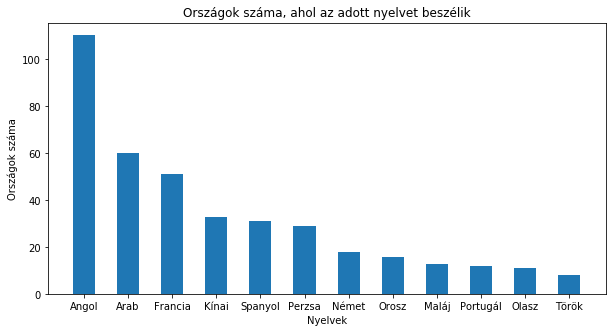
\includegraphics[width=150mm, keepaspectratio]{figures/languagesInCountries.png}
\caption{Országok száma, melyekben az adott nyelvet beszélik. \cite{nyelvekvilaga}}
\end{figure}

Számos nyelvet beszélnek világszerte az angol mellett, sokak számára viszont az angol nem az anyanyelvük, estleg egyáltalán nem beszélik azt. Beszédfelismerés során tehát szükséges egyéb hivatalos nyelveket is vizsgálni és kutatni.

Az orosz több mint 140 millió ember anyanyelve és további 110 millióan használják az oroszt második nyelvként\footnote{Az orosz nyelv, Wikipedia \url{https://hu.wikipedia.org/wiki/Orosz_nyelv}}, így az orosz nyelv igen fontos szerepet tölt be a nemzetközi porondon. Az 1.1-es ábrán látható, hogy elterjedt nyelvnek számít több országban is. Az end-to-end technológia és a neurális hálók által nyújtott lehetőségek megkönnyítik a nyelvek közti átállást, így egy angoltól eltérő nyelv vizsgálata és kutatása gördülékenyen megvalósítható egy angol nyelvű példa alapján.

\section{Diplomaterv felépítése}

A követelmények elemzése fejezetben a sarkalatos pontok kerülnek részletezésre, kifejtésre. Ezen pontok kidolgozásának lehetőségei, esetleges nehézségei kerülnek említésre a felsorakoztatva a tervezés előtt felmerült, megvalósított és elvetett ötleteket.

Az end-to-end beszédfelismerés elmélete rész a beszédfelismerés teóriájával foglalkozik, különösképp kitérve a neurális hálókat alkalmazó implementációra és azok alapjaira. Továbbá tartalmazza az eddigi legjobb megoldásokat, melyeket össze is hasonlít, röviden értékelve azok sikerességét. A levonható következtetések fényében felvázolja a fejlesztés kiindulási alapjának tekinthető állapotot és tervezésbeli döntéseket.

A tervezés és implementáció fejeztet magába foglalja az előzetes döntéseket, a lehetséges kísérletek várható eredményét. A döntési lehetőségeket, értékelve és az azok mögötti ötleteket, esetleges alternatívákkal kiegészítve. A végső soron választott megoldások alátámasztása és indoklása is megjelenik a részben.

Az összefoglaló tartalmazza az elért eredmények bemutatását, azok értékelését és a végső következtetések levonását, illetve a további kutatási lehetőségek felvázolását.
%----------------------------------------------------------------------------
\chapter{A követelmények elemzése}
%----------------------------------------------------------------------------

\section{Beszédfelismerés bemutatása}

Az irodalomkutatás során az end-to-end alapú beszédfelismerést különböző források, cikkek, internetes blogok és papírok alapján végezni. Mivel egy egészen új és feltörekvő megközelítésről van szó, célszerű a forrásokat megvizsgálni, összevetni az azonos témáról írtakat az alátámasztás és a könnyebb értelmezhetőség végett.

A neurális hálók működésének bemutatása elengedhetetlen a szerepük nyomán a beszédfelismerésben. Fontos kitérni az end-to-end alap mivoltára, ennek előnyeinek és hátrányainak bemutatása az eddig bevált, hagyományos módszerekkel szemben.

Érdemes az elméleten túl a potenciálisan felhasználható megoldásokat részletesen megismerni, melyek implementálhatók a későbbi tervezés során a jobb eredmények végett.

\section{Korszerű architektúrák és tervezés}

Többféle neuronhálós architektúrák léteznek különböző feladatokra, így a beszédfelismerésre is. Felderítésük, előnyeik és hátrányaik megismerése és összevetésük az irodalomkutatás során végezhető el. 

A neurális hálók természetüknél fogva igen összetettek, ezért gyakori az egyes rendszerek magas erőforrásigénye, melyeket a erőforrásszűkében akár kivitelezhetetlen is lenne használni. Ezért célszerű, hogy olyan architektúrát válasszunk, ami az előzőek alapján optimális teljesítményt nyújt, azaz látványos és felhasználható eredmények elérésére képes a lehető legrövidebb idő alatt a legkevesebb erőforrást felhasználva. A rövid idő alatt lefutó modellek a tesztelési fázist is nagyban felgyorsíthatják, így az idő szerepe kulcsfontosságú, míg természetesen fontos és nem elhanyagolható a pontosság is.

Kezdetben angol nyelven célszerű tesztelni az megtervezett architektúrát és az egyes paramétereinek pontosítását, mivel angol nyelven rengeteg eredmény érhető el, ezáltal összevethetőek az elért eredmények. Ha egy megtervezett rendszer működésének megítélése angol nyelvű adatok alapján megfelelő akkor már célszerű áttérni az orosz nyelvre. 

\section{Orosz nyelvű implementáció}

Egy angoltól eltérő nyelvre való áttéréskor el kell végezni annak a vizsgálatát, hogy az újabb nyelv milyen különbségeket rejt. Egy gyakori eltérés az ábécé, de előfordulhatnák más előfeldolgozásbeli különbségek is. Ha egy keretrendszer angol nyelvre van optimalizálva, előfordulhat, hogy ezeket a finomításokat el kell vetni és egy általános megközelítést kell alkalmazni az új nyelv tanítása során.

A célnyelvi adatokat különböző forrásokból lehet begyűjteni. Mivel az adatbázisok csak nyíltak lehetnek, ezért ezek megbízhatóságát meg kell vizsgálni akár szúrópróbaszerűen akár más felhasználók véleménye alapján. Az adatok mérete mind a neurális modellek tanítási ideje mind tárhelykapacitás miatt nem szabad, hogy túl nagy legyen, meg kell találni az optimális mennyiséget.

Tanítás során a jobb eredmény elérése érdekében alkalmazható a transfer-learning, ami egy elterjedt tanítási módszer neurális hálók használata során. Ez a folyamat egy adott architektúrájú, előre tanított modell továbbtanítását foglalja magába. Beszédfelismerés esetén az eredeti modelltől eltérő nyelv alkalmazásánál kihívást jelent az új nyelvre való áttérés. Szerencsére lehetőség van az előre tanított modell tetszőleges részeit átvenni, nem szükséges a nyelvspecifikus elemeket is importálni, így azok tanítása kezdődhet a többitől szeparálva, nulláról.

Célszerű az architektúra tervezésénél gondolni a szabadon elérhető előre tanított modellekre és ilyen felépítéseket is fontolóra venni és megvizsgálni, hiszen csak ezekkel lehetséges a transfer-learning alkalmazása.

\section{Optimalizálás és kiértékelés}

Az elkészült modellt ki kell értékelni, összehasonlítani más eredményekkel és véleményezni az így elért eredményt. Ezért a kiértékeléshez egy elterjedt módszert kell használni, hogy összemérhetőek legyenek az eredmények.

Lehetőség van az eredmény javítására különböző módszerekkel, melyek már ismertek a neurális hálók körében, vagy főként beszédfelismerésnél jelennek meg. Az előbbi csoportba tartozik például az augmentálás, mely folyamat során a meglévő tanítóhalmazt dúsítják különböző módszerekkel. Utóbbi csoportba tartoznak a különböző dekóderek, annak a módja hogy hogyan értelmezzük a valószínűségként kapott kimeneteket az egyes időpillanatokban, illetve a nyelvmodellek.

\section{Munka összegzése és kitekintés}

Befejezésképp kerül sor a kitűzött feladatok sikerességének bemutatására, az elért eredmények részletezéséve és az esetleges kudarcok a zsákutcák leírására. További, ki nem próbált lehetőséget és fejlesztési ötletek javaslása is fontos a munka folytathatósága végett, indokolva, hogy miért is jelenthetnek fejlődést az eredményekben és hogy ezek miért nem lettek megvalósítva, kipróbálva.
%----------------------------------------------------------------------------
\chapter{Az end-to-end beszédfelismerés elmélete}
%----------------------------------------------------------------------------

\section{Hagyományostól az end-to-end-ig}

A hagyományos ASR-ok (automatikus beszédfelismerők) több elemből álló, összetett rendszerek, melyek manapság igen pontosan meg tudják állapítani mi volt az eredetileg elhangzott szöveg, és leképezik azt írásos formába. Az egyik legelterjedtebb a HMM (Rejtett Markov Modell) alapú beszédfelismerő rendszer. A rendszernek több eleme is van: egy dekóder mely tartalmaz egy nyelv modellt, akusztikus modelleket és egy kiejtési szótárat is, illetve tartalmaz egy elemet, mely a bemeneti hangból a kiemeli jellemzőket, átalakítja őket a rendszer által kezelhető formájúvá. A HMM-en alapuló rendszerek fő eleme a Viterbi algoritmus \cite{viterbi}, mely dinamikus programozást alkalmazva találja meg a legjobb illeszkedést a bemeneti szöveg és az adott beszéd modell közt.

A rendszer különböző elemei erősen függenek egymástól. Ha az egyik nem rendeltetés szerűén működik és rossz kimenetet ad, akár saját vagy egy korábbi elem hibájából kifolyólag az befolyásolja a többi elemet is, így elrontva, torzítva a kapott végeredményt. Az egyes elemeket külön-külön kell kalibrálni, tanítani és tökéletesíteni.

Ezzel szemben, a napjainkban egyre inkább népszerű, E2E (end-to-end) alapú beszédfelismerő rendszerek sokkal egyszerűbb struktúrájúak, kevesebb különálló elemet igénylő megközelítést nyújtanak. Bizonyos szituációkban, ahol egy specifikusabb szövegkörnyezetben, pl. pénzügyi vagy jogi, elhangzó szavak azonosítása a cél, már a hagyományos ASR rendszereknél is pontosabb eredményeket képesek produkálni.

Az E2E rendszerek mély neurális hálókon alapszanak, közvetlen bemenetük a nyers hang, kimenetük pedig a becsült szöveg. Természetesen a neurális háló bemenetéhez a pontosabb eredmény végett a hangot előre fel kell dolgozni, amit pre-processing-nek, előfeldolgozásnak, neveznek. A háló kimenete pedig az egyes bemeneti időegységekre becsült karakterek valószínűségeinek mátrixa melyekből ki kell nyerni a végső, feltételezett szöveget.

\section{A beszédfelismerés lépései}

\subsection{Előfeldolgozás}

A beszéd előfeldolgozása az első fontos lépése a beszédfelismerő rendszereknek. Vannak törekvések, melyekben a E2E neurális hálónak közvetlenül a nyers, feldolgozatlan hanganyagot adják meg és ez alapján tanítják\cite{Zeghidour2018}, ezáltal még inkább tisztán a neurális háló működésére támaszkodva. Egyelőre ennek a megközelítésnek az eredményei messze elmaradnak a hang előfeldolgozásával elérhető SOTA modellek pontosságától.

A két fő megközelítés többnyire hasonló, apró eltérésekkel. Az egyik legelterjedtebb és bevált átalakítás a spektogram.

Ahogy az 1. ábrán is látható, a spektogramm három tengely mentén reprezentálja az adatot. A vízszintes tengelyen az idő, míg a függéleges tengelyen a frekvencia van megadva. Van továbbá egy harmadik tengely is, ami színnel van jelölve és mértékegysége a decibel. Ez a jel amplitúdója, ami az adott időpillanatban, adott frekvenciához tartozik és a szín intenzitása reprezentálja a kép pontjain mértékét.

A szokványos spektrogrammon kívül használatos még a MFCCs (Mel-Frequency Cepstral Coefficients) is. Felépítése hasonló a spektogramméval, viszont a frekvencia helyett az MFC koefficiens \cite {mfcc} értéke van az függőleges tengelyen. Ez a Mel skála, amely úgy van megválasztva, hogy a skálán egyelő távolságra lévő hangok az emberi fül számára is hasonló távolságúnak, azonos léptékben különbözőnek, tűnjenek. A frekvenciához képest egy lényeges változást jelent, hiszen az ember számára könnyen hallható kisebb frekvenciákon, például az 500 Hz és 1000 Hz közötti különbség, míg 6500 Hz és 7000 Hz között már kevésbé számottevő az eltérés. Az MFCC nagyságrendekkel kisebb a frekvencia értéknél így lényegesen befolyásolhatja a neurális háló tanulási folyamatát.

Az előfeldolgozott jelet időegységekre bontjuk, melyek már a neurális háló bemenetét képzik. A kimeneten az egyes időegységekre kapott predikciókból pedig összeállítható a feltételezett szöveg.

\begin{figure}[!ht]
\centering
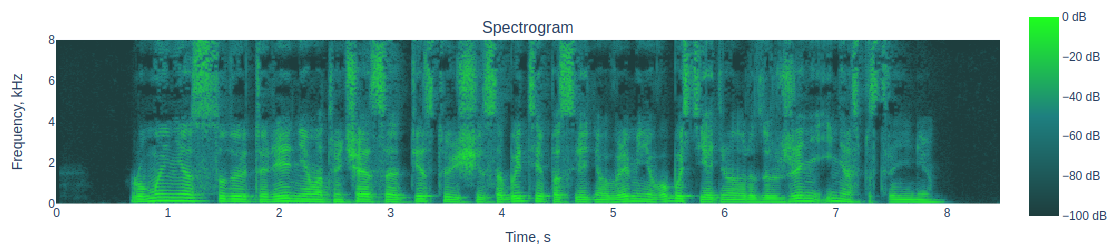
\includegraphics[width=150mm, keepaspectratio]{figures/spectogram.png}
\caption{Spektogram.}
\end{figure}

\subsection{Neurális hálók}

A neurális hálók az emberi idegek működésének mintája alapján modellezett láncolatok. Számos különböző, komplex feladat megoldására előszeretettel alkalmazzák őket. Röviden összefoglalva három fő alkotó részből állnak. Egyik a bemenet, például egy kép esetén a pixelek, beszédfelismerés esetén az egyes időpillanatokhoz tartozó értékek vektor formában. Spektogram esetén az időpillanathoz tartozó vektor egyes elemei a frekvenciát jelképezik és az elemek értéke pedig a hangerősséget.

A neurális háló közbülső, rejtettnek, nevezett része tetszőleges méreteket ölthet. Az egyes rétegek pontjai mindig az előző réteg pontjaival vannak összekötve úgy nevezett súlyok segítségével. Az újabb rétegek pontjainak értékét az abba befutó súlyok, illetve a súlyok és kiinduló pontjuk szorzatainak az összegével számítjuk. A pontok végső értéke még egy aktivációs függvénynek nevezett kiértékelésen is keresztül megy, mielőtt a következő réteg értékeit kiszámíttatnánk vele. Az aktivációs függvények igen eltérőek lehetnek, egy népszerű függvény a ReLU, ami a 3.2-es ábrán látható. Ezeket a pontokat neuronoknak szokás nevezni, innen ered a neurális háló kifejezés. A háló tanítása során ezen súlyok értékét módosítjuk úgy, hogy a legoptimálisabb, számunkra kedvezőnek vélt eredményt kapjuk.

\begin{figure}[!ht]
\centering
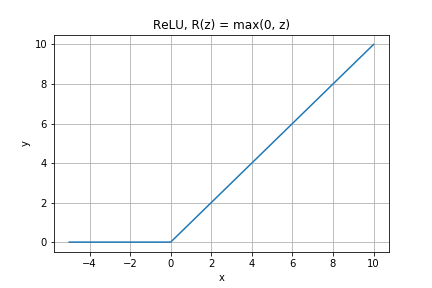
\includegraphics[width=120mm, keepaspectratio]{figures/ReLU.png}
\caption{A ReLU aktivációs függvény.}
\end{figure}

Az utolsó réteg a kimeneti réteg, ahol az eredményt kapjuk meg. A kimeneti réteg lehet regresszív, egy előre meg nem határozott, tetszőleges érték, vagy a mint a mi esetünkben klasszifikáció, amikor előre meghatározott címkék (label-ek) valószínűségére vagyunk kíváncsiak. Legegyszerűbb estben a legvalószínűbb címke kerül kiválasztásra válaszként, de a beszédfelismerésnél a később taglalt CTC alapú loss számítás működéséhez az egész kimeneti mátrix vizsgálata szükséges.

A valószínűség kiszámításához a softmax \cite{softmax} függvényt szokás használni, ami szintén egy aktivációs függvény. A függvény egy vektor bemenetet megkapva normalizálja a vektor egyes értékeit úgy, hogy azok új értékei 0 és 1 közé essenek, miközben az összegük pontosan 1-et adjon. A softmax függvény, ahol x a bemeneti vektort jelöli, míg i és j a vektor egyes elemeinek a sorszámát:

\begin{align}
softmax(x)_i = \frac{exp(x_i)}{\sum_{j}^{ }exp(x_j))}.
\end{align}

Neurális hálók egyik leggyakoribb, a munkák során általam is alkalmazott, tanítási módszere a felügyelt tanítás. Ez azt jelenti, hogy először például egy tanítatlan, véletlenszerűen inicializált, hálóból kiindulva kiértékeljük egy tetszőleges bemenetre a végeredményt. Majd a végeredmény helyességétől függően változtatjuk a súlyok értékét a hálóban: azon súlyokat melyek egy rossz eredmény nagyobb valószínűségéhez járultak hozzá büntetjük, úgy csökkentjük az értéküket, hogy kevésbé befolyásolják a végeredményt, míg azokat melyek egy jó eredmény pozitív értékéhez járultnak hozzá növeljük. Ezt a folyamatot szokás backpropagation-nak nevezni. A büntetés mértéke is létfontosságú, hiszen fontos, hogy ne csak az adott bemenetre tudjon pontos végeredményt adni a háló, hanem általánosan is pontos legyen. 

Az egyik legegyszerűbb réteg típus a Dense (sűrű) vagy más néven Fully Connected, ahogy a neve is utal rá az egyes neuronok a súlyokkal sűrűn vannak összekötve. Ez azt jelenti, hogy az adott réteg mindegyik neuronja össze van kötve az előző réteg összes neuronjával súlyok által. Több Dense réteg is követheti egymást, mely esetben az adott réteg összes neuronja össze van kötve a következő réteg összes neuronjával is.

Az E2E-nél használt leggyakoribb neurális háló réteg fajták az rekurrens (RNN) és konvolúciós (CNN) rétegek. Ez utóbbit elterjedten használják a különböző képfelismerő feladatok megoldásánál is.

Lényegesen összetettebb a Dense rétegnél a konvolúciós réteg\cite{cnn}, melynél egy, a teljes bemenetnél kisebb, kernel-t (vagy filtert) mozgatunk végig a bemenet elemein és kiértékeljük az általa lefedett értékeket. A lefedett számokat a kernel velük fedésben lévő értékével összeszorozzuk, ezek az értékek főként a -1, 0 és 1, majd a kapott eredményeket összeadjuk. Ezt követően a kernel-t egy megadott értékkel, a stride-al mozgatva kiértékeljük a következő, kernel által lefedett számokat. A konvolúció végezhető egy vagy több dimenziós bemeneten, különböző kernel-ekkel párhuzamosan is, kép esetén például három csatornás képen, ahol a piros kék és zöld értékek külön csatornákon vannak reprezentálva. Egy opcionális lépés, hogy a bement széleit feltöltjük-e nullásokkal, ez az úgy nevezett zero padding. Ennek célja, hogy ugyan akkora legyen a kimenet, mint a padding nélküli bemenet volt. Ezen kívül is szükség lehet padding-re például egy 5x5-ös kép esetén, ha a kernel mérete 3x3 és a stride 3, akkor ki kell tölteni a kép széleit, hogy minden bemeneti értéken legalább egyszer végig menjen a kernel.

Egy CNN-hez kapcsolódó, kernellel rendelkező rétegtípus a pooling réteg, mely kifejezetten az adat méretének csökkenését szolgálja. Ezzel a célja a számítási kapacitás csökkentése, miközben minél inkább megőrzi az adatban rejlő információt. Két használt pooling típus a max vagy average pooling. Előbbinél a kernel által befoglalt értékek maximumát választja, míg utóbbinál az átlagukat egy számra csökkentve a kernel által közrefogott értékeket.

A konvolúciós vagy pooling rétegek működésükből adódóan csökkenthetik a kimenetük méretét, ezáltal ismerni kell annak pontos dimenzióját, a következő réteghez kapcsolódó számítások végett. A kimenet méretét a következő képlettel lehet kiszámolni, ahol ’O’ a kimenet mérete, ’W’ a bemenet mérete, ’P’ a padding mérete, ’K’ a kernel mérete és ’S’ a stride:

\begin{align}
\mathbf{O}&=\frac{\mathbf{W}-\mathbf{K}+\mathbf{2P}}{\mathbf{S}+\mathbf(1)}.
\end{align}

A rekurrens rétegek\cite{rnn} egyik legérdekesebb tulajdonsága, hogy nem csupán a bemeneti súlyaikat használják a neuronok kiértékeléséhez, így felhasználva a korábban tanultakat, hanem emlékeznek a korábbi neuron értékeikre is, melyek szintén befolyásolják az aktuális bemenetre kapott eredményt. Beszédfelismerés esetén ezt úgy is el lehet képzelni, hogy ha például elhangzik egy magánhangzó, akkor utána nagy valószínűséggel egy mássalhangzót várunk, ennek fényében, sikeres tanítás esetén, a mássalhangzókat részesíti előnyben egy azt megelőző magánhangzó után. Korábbi időpillanatok, állapotok tehát hozzájárulnak egy újabb állapot kiértékeléséhez a rekurrens rétegben, ahogy ez a 3.3-as ábrán is látható.
 
\begin{figure}[!ht]
\centering
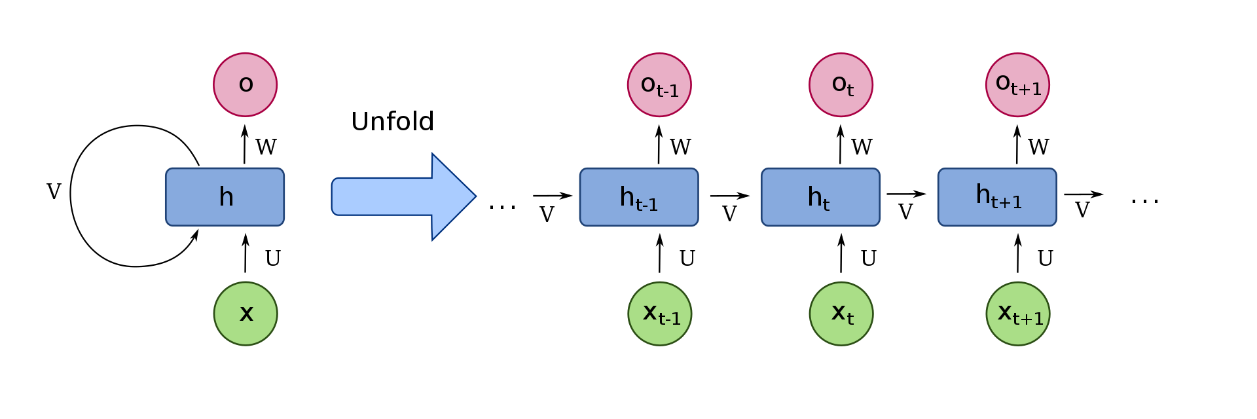
\includegraphics[width=140mm, keepaspectratio]{figures/rnn.png}
\caption{A rekurrens réteg "kigörgetve" \cite{rnn}.}
\end{figure}

Két altípusa a rekurrens hálóknak az LSTM és GRU (Long Short Term Memory, Gated Recurrent Unit). Ezek a típusok hasonló elveken működnek, a különbség a neuronok korábbi értékeinek újabb értékekre történő ráhatásának számítási módjában rejlik. Az LSTM [7] fő célja, hogy kijátssza a hagyományos rekurrens hálók egyik legnagyobb problémáját, azt, hogy a régebbi bemenet súlya nincs hasonló fontossággal kezelve, mint a jelenlegi bemenethez közelebbi érték. Könnyen belátható, hogy fontos lehet egy mondat végi szót vizsgálva, hogy mi volt a szó a mondat elején, akár a vizsgálandó mondat elemet megelőző néhány szónál is. Az LSTM kapukat használ annak megelőzése céljából, hogy egy korábbi értékelés elvesszen, ezáltal kezelhetetlenné téve annak beleszámítását az újabb értékelésnél.

A GRU egy LSTM-hez hasonló újabb fejlesztésű réteg. Egyik fő tulajdonsága, hogy kevesebb elemet tartalmaz, így kevesebb paramétert használ, csökkentve a neurális háló komplexitását, ezáltal a szükséges számítási időt is.

Megemlítendő még a Bi-directional (két irányú) réteg, amely mögött az a gondolat húzódik meg, hogy ne csak a múltbéli bemenetek befolyásolják az adott bemenetünket, hanem a jövőbeliek is. Két rekurrens réteget használ, melyek ellentétes irányban haladnak egymással, így tetszőleges kiértékelésnél használhatóak a korábbi, illetve elkövetkezendő neuronok eredményei is.

A rekurrens rétegek nagy léptékben meg tudják emelni a modellek paraméterszámát, ezért használatuktól igyekeztem tartózkodni, mivel az architektúra kiválasztásának fő szempontjai az alacsony paraméterszám, és a gyors kiértékelési és tanítási sebesség voltak.

\subsection{CTC dekódolás és loss számítás}

A CTC (Connectionist Temporal Classification) \cite{ctc} funkciója a kimenet dekódolása, a válasz kiértékelése, mely folyamán átalakítja a kimenetet a megadott címkék valószínűségi szekvenciájára és a tanításhoz szükséges hiba, a loss kiszámítása. A címkék lehetnek az egyes karakterek, amik egy adott nyelvben előfordulhatnak. Ez esetben a CTC kiértékeli, hogy melyik betű vagy egyéb karakter hangzott el adott időpillanatban, adott bemenetre [8]. Ereje abban rejlik, hogy nincs szükség a kiértékelésnél a kimeneteket egyenként, karakter szinten összekötni az elvárt szöveggel, elegendő a kimeneti szöveget megadni, azt, amit kapni szeretnék az adott bemenetre. Másik fontos előnye, hogy a felismert szöveget nem szükséges külön feldolgozni, mivel átalakítja azt a végleges, feltételezett formára. Feldolgozza, hogy egy hosszú hang esetén, mint az ’ú’ több időpillanaton keresztül is hallatszik az ’ú’ betű, de nekünk a végeredményben csak egy darab ’ú’ szükséges.

Felmerülhet egy probléma az összevonással, amikor olyan egymást követő betűket vonunk össze, melyek a szóban külön szerepelnek, mint például az ’ellentét’ szóban. Ennek elkerülése végett bevezet a CTC egy üres karaktert, ami nem egyenlő a szóközzel, és ezt olyan időegységekhez helyezi, ahol nem ismerhető fel betű a megadott szótárból, karaktergyűjteményből. Az ilyen üres karakterrel elválasztott betűket nem fogja összevonni kiértékeléskor.

A neurális háló által végzett kiértékelés után az ember által feldolgozható kimenet megszerzéséig szükség van még a karakterek összeillesztésére. Ehhez különböző elven működő dekódolókat használunk. Az egyik legalapvetőbb dekódolási algoritmus a best path eljárás. Két dolgot végez: kiszámolja a legvalószínűbb útvonalat a kapott kimeneti időegységeken át, majd eltávolítja az egymást követő azonos karaktereket, melyek közt nem található az üres karakter. Végül az üres karaktereket is eltávolítja, így eredményezve a végső predikciót.

További feladata a neurális háló tanításához használt loss kiszámítása \cite{ctc_sid}. A hiba számítása során a szempontunkból lényegtelen milyen karaktersorozattal jut el a végeredményhez, csupán az a cél, hogy pontosan az adott kimenetet eredményezze. A loss-t tehát úgy számítja, hogy megnézi az összes olyan karaktersorozat valószínűségét, melyből megkaphatja a kívánt eredményt és összegzi őket. Ezáltal az eredeti GT (Ground Truth) szöveg valószínűségi értéke magas, hogyha a megszerzéséhez szükséges kombinációk értékének az összege magas.

A tanításhoz szükséges CTC loss számítása a 3.3-as, 3.4-es és 3.5-ös képeltek alapján történik, ahol GT az elvárt szöveg, X az egyes akusztikus keretek, C egy adott karaktersorozat és $c_t$ egy adott karakter adott időpillanatban.
\begin{align}
CTC loss&=-\log{P(GT | X)}.
\end{align}

Összes lehetséges helyes karaktersorozat valószínűségének az összege:
\begin{align}
P(GT | X)&=\sum_{C=A(GT)} P(C | X).
\end{align}

Egy adott, helyes karaktersorozat valószínűsége:
\begin{align}
P(C | X)&=\prod_{t=1}^{T} y(c_t, t)).
\end{align}

A neurális háló kimenetén megadja a megadott karakterek valószínűségi mátrixát minden időpillanatban. Mivel a loss kiszámítása a GT szöveg összes lehetséges illeszkedés alapján történik, ezért lényegtelen, hogy hogyan helyezkedik el pontosan a megadott hanganyagban. A fenti képletekkel kiszámítható egy tanító szöveg valószínűsége a megadott GT és a neurális háló által adott valószínűségi mátrix alapján. A cél, hogy aképpen tanítsuk a hálót, hogy magas valószínűségeket kapjunk az elvárt ground truth kimenetkre. Ezt úgy lehet elérni, hogy minimalizáljuk a tanítóadathalmazra kapott loss értéket, ahol a loss a valószínűségek logaritmikus értéknek negatív összege. Az egyes loss értékek kiszámításához a valószínűség kiértékelése után elég annak logaritmusát venni, majd negálni az eredményt. A neuron háló tanításához a loss grádiensét kell kiszámolni, azt az értéket amivel a többdimenziós térben a legnagyobb csökkenést lehet elérni, és az egyes paramétereket, súlyokat frissíteni vele\cite{ctc}.

\section{Létező megoldások}

A beszédfelismerő rendszereket pontosságuk alapján tudjuk rangsorolni. Egy nemzetközileg elismert pontossági mérőszám a WER (Word Error Rate). Ezt a pontosságot szokás szerint egy publikusan elérhető, angol nyelvű hangoskönyv felolvasásokat tartalmazó adatbázison, a LibriSpeech-en\footnote{LibriSpeech oldala: \url{http://www.openslr.org/12/}} mérik.

Különböző, alacsony hibaarányú modellek léteznek, de ez egyik lekiemelkedőbb közülök az Nvidia QuartzNet modellje, mely alacsony számú paraméterek mellett képes igen nagy precíziót fenntartani. Míg a QuartzNet bonyolultsága, paramétereinek a száma csupán töredéke a legtöbb SOTA modellének\footnote{Az Nvidia ismertető oldala: \url{https://developer.nvidia.com/blog/develop-smaller-speech-recognition-models-with-nvidias-nemo-framework/}}, a WER száma megközelíti azokét (3.1-es táblázat).

A modellekben elterjedt a konvolúciós- (CNN) és rekurrens neurális rétegek  (RNN) használata.

\begin{table}[ht]
	\footnotesize
	\centering
	\begin{tabular}{ p{2.5cm} p{2.5cm} p{2.5cm} p{1.5cm} p{1.5cm} p{1cm} }
		\toprule
		\textbf{Model} & \textbf{Aug} & \textbf{LM} & \textbf{clean WER(\%)} & \textbf{other WER(\%)} & \textbf{Million Parameters} \\
		\midrule
		wav2letter++\cite{w2l} & Speed Perturb & ConvLM & 3.26 & 10.47 & 208 \\
		\hline
		LAS\cite{las} & SpecAugment & RNN & 2.5 & 5.8 & 360 \\
		\hline
		Time-Depth Separable Convolutions\cite{timedepth} & Dropout, Label Smoothing & N/A (greedy) & 5.36 & 15.64 & 37 \\
		&  & 4-gram & 4.21 & 11.87 &  \\
		&  & ConvLM & 3.28 & 9.84 &  \\
		\hline
		Multi-Stream Self-Attention\cite{attention} & Speed Perturb & 4-gram & 2.93 & 8.32 & 23  \\
		&  & 4-LSTM & 2.20 & 5.82 &  \\
		\hline
		QuartzNet-15x5\cite{quartznet} & Spec Cutout, Speed Perturb & N/A (greedy) & 3.90 & 11.28 & 19 \\
		&  & 6-gram & 2.96 & 8.07 &  \\
		&  & Transformer-XL & 2.69 & 7.25 &  \\
		\bottomrule
	\end{tabular}
	\caption{Az egyes SOTA beszédfelismerő modellek és paramétereik.}
\end{table}

%----------------------------------------------------------------------------
\chapter{Tervezés}
%----------------------------------------------------------------------------

\section{Tervezés, döntési lehetőségek értékelése}

\subsection{Fejlesztési nyelv}

A Python napjaink egyik legelterjedtebb programozási nyelve. Egy könnyen programozható és átlátható, interpretált nyelv, melyben a megírt program kódot a Python értelmező sorról-sorra értelmezi és futtatja, nincs különválasztva a forrás és a fordított kód. Deep learning körökben is dominál a Python nyelv, rengeteg deep learning toolkit erre a nyelvre épít, így választásom a fejlesztéshez természetesen a Python nyelvre esett.

\subsection{NeMo}

A neurális hálók komplikáltságából adódik, hogy pontos és precíz implementációjuk igen bonyolult és időigényes. Emiatt célszerű a már meglévő, bejáratott és bizonyított lehetőségeket használni, így felgyorsítva a fejlesztési folyamatot és javítva a potenciálisan elért eredményeket. Több deep learing platform is található az internetet, mint például a Tensorflow vagy PyTorch. Az Nvidia által fejlesztett NeMo\footnote{NeMo toolkit, \url{https://github.com/NVIDIA/NeMo}} egy olyan összetett és folyamatosan karbantartott toolkit, melynek segítségével különböző mesterséges intelligencia alapú társalgási, beszéddel kapcsolatos applikációkat, alkalmazásokat készíthetünk. Munkám során ennek fényében a NeMo toolkit-et használtam.

Az alap koncepcióját a toolkit-nek az úgynevezett Neurális Modulok alkotják. Ezek a modulok lehetnek például adat rétegek, kódolók, dekóderek, nyelv modellek vagy loss függvények. A modulok ereje abban rejlik hogy egymáshoz viszonyítva tetszőlegesen építhetők, cserélhetők, törölhetők. Egy egyszerű módosítással kicserélhető például a loss számításához használt függvény anélkül, hogy a kódot a többi modulban módosítani kéne.

Az 3.1-es táblán látható modellek közül az Nvidia fejlesztette a legkevésbé számításigényeset, mely figyelemreméltó eredményeket produkál. Ez a QuartzNet modell, ami az alacsony paraméterszáma ellenére SOTA eredményeket ér el. A felsorolt okokból kifolyólag a fejlesztési folyamat elvégzéséhez választásom a NeMo toolkit-re esett.

\subsubsection{PyTorch}

A NeMo a PyTorch nevű, Facebook-os kutatók által fejlesztett, mesterséges intelligencia fejlesztésére szakosodott nyílt forráskódú keretrendszerre épít. A PyTorch a TensorFlow-nál magasabb szintű, könnyebben kezelhető keretrendszer, mely egyre inkább elterjedtté válik a kutatók és fejlesztők körében.

\subsubsection{QuartzNet}

A kísérleteimet QuartzNet architektúrájú modellekkel elvégeztem, a korábban említett alacsony paraméterszáma és magas precizitása végett. Az architektúra (4.1-es ábra) nagyban hasonlít egy másik Nvidia által fejlesztett architektúrához, a Jasper-hez. A modell B darab blokkból áll. Egy opcionálisan beállítható dropout modul is megjelenhet a modellben, illetve CTC loss függvény számítás található benne. A már említett blokkok további, R darab blokkból állnak, melyek konvolúciós rétegekből, batch normalizálókból és ReLU aktivációs függvényből épülnek fel. Ezáltal a QuartzNet pontos felépítésére QuartzNet BxR alakban szokás hivatkozni. A legnagyobb Nvidia által készített a Quartznet 15x5, mely 18.9 millió paraméterből áll, amit kiterjedten használtam a  kísérleteim során.

A QuartzNet a Jasper-től a konvolúciós rétegeinek a típusában tér el. A sima egy dimenziós konvolúciós réteg helyett, egy dimenziós time-channel separable konvolúciós rétegeket használ \cite{quartznet}. Ennek a fő tulajdonsága, hogy jóval kevesebb paramétert használ az eredeti koncepciónál. Ennek köszönhetően mélyebb hálókat lehet készíteni nagyobb konvolúciós kernelekkel anélkül, hogy a a paraméterek száma, ezáltal a szükséges számítása kapacitás túlzottan megnövekedne.

\begin{figure}[!ht]
\centering
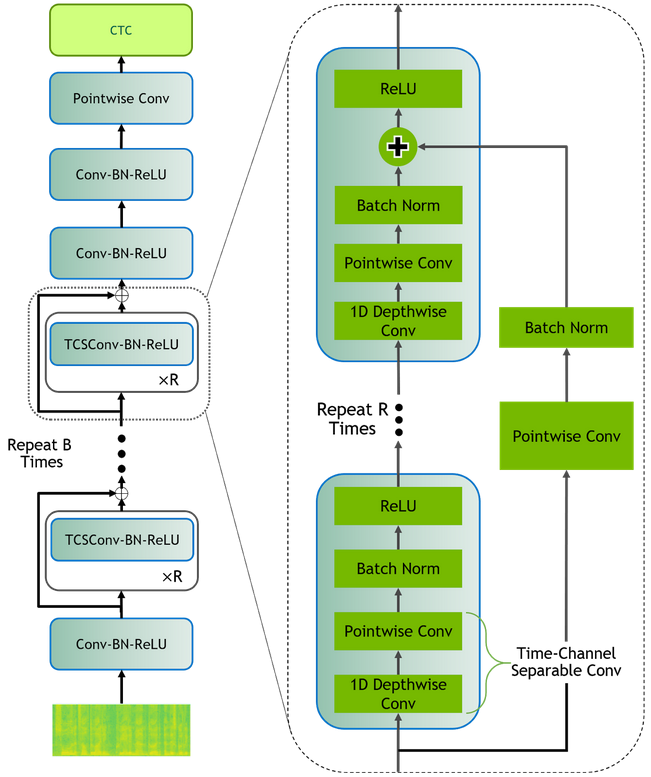
\includegraphics[width=150mm, keepaspectratio]{figures/QuartzNet-architecture.png}
\caption{QuartzNet architektúra. \cite{nemo}}
\end{figure}

\subsection{TensorBoard}

Az eredmények kiértékeléséhez és nyomon követéséhez a TensorBoard-ot, a TensorFlow egy vizualizációs toolkit-jét használtam. Több funkcióval is rendelkezik, mint például a súlyok időbeni változásának vizualizációja, illetve a tanítóadatok, képek, szöveg vagy hang anyag kijelzése. Számomra a legfontosabb tulajdonsága az egyes metrikák, a loss és a pontosság, a WER, értékének változásának nyomon követése.

A TensorBoard könnyedén indítható a következő parancs kiadásával: $tensorboard --logdir ~/lightning-logs$ , ahol a logdir kapcsoló adja meg melyik könyvtárban keressen TensorBoard kompatibilis log-okat, event-eket. A főkönyvtárban egyes almappáiban kell elhelyezni a tanítás során előállított event-eket, így a Tensorboard különálló tanításként ismeri fel őket. A szükséges event-ek előállítása könnyedén végezhető a NeMo toolkit segítségével, mely támogatja a megfelelő callback függvények használatát, amik az event-ek batch-enkénti frissítsét tesznek lehetővé. A callback függvény egyszerűen bővíthető szükség szerint.

\begin{figure}[!ht]
\centering
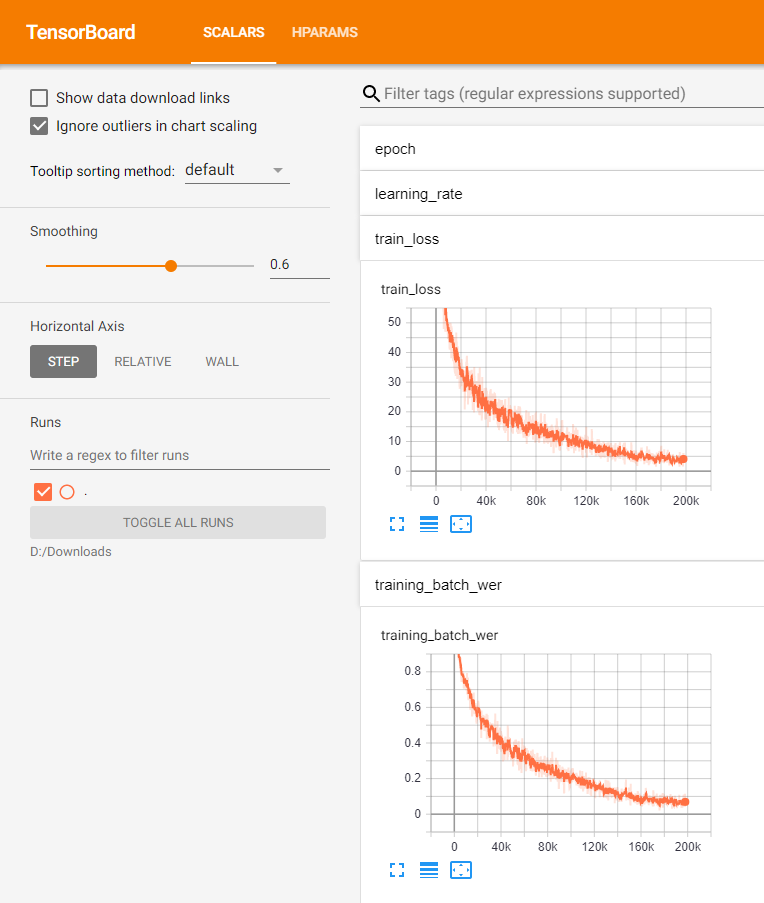
\includegraphics[width=150mm, keepaspectratio]{figures/tensorboard-example.png}
\caption{Lokálisan futtatott TensorBoard.}
\end{figure}

\section{Angol, majd orosz}

Kezdetben a tesztelést az egyik leggyakoribb nyelven, az angolon, végeztem. Ennek oka főként az volt, hogy megbizonyosodjak a modellem és a NeMo beállításainak sikerességéről, hogy megfelelő eredményeket tudok elérni elterjedt, kisebb adatbázisokon. Másfelől a modellem hiperparamétereit, mint például a learning rate, optimalizáltam, és az orosz nyelven történő kísérletezésnek a legbiztatóbb beállításokkal tudtam nekiállni.

Az angol nyelvű eredményeket viszonyításként is fel tudtam használni az végső orosz eredményekkel való összehasonlításánál, ahol a nagyságrendileg azonos mennyiségű orosz adatoknak az angoléhoz hasonló eredményeket kellett produkálniuk.

\subsection{Google Colab}

A NeMo-val való ismerkedéshez felhasználtam egy, az Nvidia által írt, jupyter notebook-ot\footnote{Tutorial notebook, \url{https://github.com/NVIDIA/NeMo/blob/main/tutorials/asr/01_ASR_with_NeMo.ipynb}}, melyet könnyedén és ingyenesen lehet Google Colab-ból\footnote{Google Colab, \url{https://colab.research.google.com/notebooks/intro.ipynb}} futtatni. A Colab ingyenes hozzáférést nyújt GPU erőforrásokhoz, ahol egyenesen a böngészőből futtatható a Python kód és az eredményeket akár le is lehet tölteni. Csupán be kell importálni a Colab környezetbe a github-on elérhető notebook-ot a az URL megadásával, majd tömbönként futtatható a kód, melyhez magyarázat is tartozik.

Sajnos a Colab bizonyos órán belül felfüggeszti a munkamenetet, illetve a nagy mennyiségű adatok munkamenetenkénti le- és feltöltése időigényes. Ezért főleg a kisebb, rövidebb adatbázisokon, mint például az AN4-en, lehetséges a kísérletezés és a toolkit-tel való ismerkedésen túl nem jelent megoldást.

\section{Adatbázisok}

A megfelelő modell megtalálásához két darab angol nyelvű adatbázist is használtam. Mikor elégedett voltam az eredményekkel és megbizonyosodtam, hogy sikeresen beállítottam a NeMo toolkit-et is, áttértem az orosz nyelvű modell fejlesztésére.

Az adatbázisokon belül három különböző típusú, egymástól független adathalmazt szükséges megállapítani. Az egyik a tanító adathalmaz, ezeket a hanganyagokat közvetlen a háló tanítására használjuk. Fontos, hogy legyen egy validációs vagy teszt adathalmaz is, amit tanítás közben használunk kiértékelésre, a tanítás általános pontosságának értékelésére. A harmadik dev adathalmaz pedig azért szükséges, mert a validációs adathalmaz pontosságát igyekszünk javítani, majd amikor ezzel elégedettek vagyunk egy tőle független adathalmazzal vizsgálhatjuk meg a végső pontosságot.

\subsection{Adatok előfeldolgozása}

Magukat a hangfájlokat is meg kell vizsgálni, egységesíteni kell a tanítás előtt. A leggyakrabban használt kiterjesztés a .wav, így én is ennek a használata mellett döntöttem. Szükség esetén az egyes hangfájlokat át kell konvertálni ebbe a formátumba a tanítás, kiértékelés előtt.

A hanganyagok mintavételezése sem elhanyagolható. A túl alacsony mintavételezés minőségi romlást, ezáltal rosszabb eredményeket okozhat, míg a túl magas mintavételezés lassítja a tanítási folyamatot és akár szintén rosszabb eredményeket produkálhat.

Az adatbázisok esetén megvizsgálandó, hogy hány beszélő hangja található benne. Minél több van benne annál általánosabban alkalmazható jobb eredményekkel.

\subsection{AN4}

Az AN4\cite{an4} vagy "census" angol nyelvű beszéd adatbázist 1991-ben vették fel a Carnegie Mellon Egyetemen. A különböző beszélők betűzve mondanak olyan adatokat mint a születési dátumuk, telefonszámuk, a nevük vagy egyéb véletlenszerűen generált, előre definiált kontroll szavak.

Az adatbázis két különböző részre van osztva, az első a tanítást szolgálja, míg a második része a tesztelést. Ez előbbi 50 percnyi beszédet tartalmaz, míg a tesztelésre szolgáló rész 6 percet. Rövidségéből adódóan gyorsan tanítható és értékelhető, mely ideálissá teszi gyors kalibrálási, beállítási feladatok megoldására.

\subsection{LibriSpeech}

A LibriSpeech egy több száz órát tartalmazó, szintén angol nyelű, hangoskönyv gyűjtemény. Ez az egyik leginkább használt adatbázis, melyet előszeretettel alkalmaznak tudományos, kutatási munkák során, hálók tanításához és ezáltal az eredményeinek ismertetésekor.

Az elérhető hanganyag fele tiszta, könnyen érthető, míg másik fele zajosabb körülmények közt lett felvéve vagy kevésbé kivehető. Külön tartalmaz tanító, teszt és dev adathalmazokat.

\subsection{Mozilla Common Voice}

A Mozilla Common Voice\footnote{Mozilla Common Voice weboldala, \url{https://voice.mozilla.org/}} egy Mozilla által indított projekt. Célja, hogy különböző nyelveken, így oroszul is, a közösség erejét felhasználva gyűjtsön anonim hanganyagokat. Bárki felveheti a saját hangját, előre meghatározott szövegeket felolvasva, illetve érvényesíthet mások által felolvasott szövegeket. A biztonság és pontosság kedvéért egy szöveget két személynek is jóvá kell hagynia.

Orosz hangból durván 100 órányi áll rendelkezésre, de tüzetesebb vizsgálat után észrevettem, hogy ebből ~10-10 óra a teszt és dev adathalmaz mérete, míg ~20 óra a tanító adathalmazé. A maradék ~60 óra nagy része azért nincs használva, mert megismételt szöveget olvasnak fel benne, vagy rövid hanganyagokat tartalmaz. A tanító adathalmazt sikerült feldúsítsam ~45 óra környékére azáltal, hogy belevettem a 100 órányi hangból az összes olyan hangot, melyek nem voltak benne sem a teszt sem a dev adathalmazokban.

% insert random data analysis here?

\subsection{További orosz adatbázisok}

Mivel a Mozilla Common Voice orosz nyelvű adatbázisa legfeljebb 45 órányi tanítóadattal rendelkezik, míg a LibriSpeech-é mely eredményeihez viszonyítani szeretnénk 100 órán lett tanítva, ezért több tanítóadatot is be kellett vonni. Egy ingyenesen hozzáférhető github-on található projektben\footnote{Ingyenes orosz adatbázisok, \url{https://github.com/snakers4/open_stt/blob/master/README.md}} több adatbázis is található, többnyire .opus formátumban. Ezek közül elsősorban a "radio2" adatbázissal dolgoztam.

Fontos megemlíteni a Mozzila Common Voice és egyéb rádiós műsorban elhangzott hanganyagok közötti lehetséges különbségeket. Míg előbbi többnyire bediktált, felolvasott szöveget tartalmaz különböző minőségben és tempóban, utóbbi kötetlenebb, tisztább minőségű beszélgetéseket is tartalmazhat.
%----------------------------------------------------------------------------
\chapter{Implementáció}
%----------------------------------------------------------------------------

\section{Tanítóadatok előkészítése}

A letöltött tanítóadatokat NeMo által értelemzhető formátumúra kellett hozni. Ez magába foglalta a fájlok konvártálását .wav formátumba. Az egyes tanítóadatok más-más formátumban (.opus, .flac, .mp3) voltak eredetileg, illetve eltérő fájstruktúrákba voltak szervezve.

A konvertáláshoz a fentiek miatt a python os könyvtárának walk metódusát használtam mellyel egy mappát rekúrzívan be lehet járni. A konvertáláshoz az ffmpeg szoftvert használtam, mivel segítségével több formátum is könnyedén konvertálható .wav formátumba.

A fájlok átalakításán kívül szükséges volt az adatok .json fájljainak elkészítése, mely megmondja, hogy melyik hangfájl hol található, milyen hosszú és mi hangzik el rajta. A NeMo-nak ezután csupán az egyes manifest-eket, .json fájlokat, kellett megadni, azzal a kiegészítéssel, hogy melyiket kívánjuk tanító vagy teszt adathalamznak használni, és a további előfeldolgozási lépéseket már autómatikusan elvégezte. Természetesen több információ tárolását is támogatja a NeMo, de ezek az adatok elengedhetetlenek.

\section{Modellek kimentése és betöltése}

A tanított modelleket el kell menteni későbbi használat végett. Két módszert is alkalmaztam. Az egyik a logoláshoz hasonlóan callback-et használ, mindig a legoptimálisabb eredményt elért epochot menti ki .ckpt fomrátumban, míg az utóbbi módszer a tanítás végén menti ki a modellt .nemo formátumban.

A mentésre a későbbi felhasználás meleltt azért is van szükség, mert a hosszú tanításokat, melyek akár 48 órán át is tarthatnak, szükséges lehet megszakítani. A megszakítás után fontos úgy betölteni a modellt, hogy az továbbtanítható legyen. A NeMo külön kezeli a modellt és a tanítást végző trainert, melykbe külön külön szükséges betölteni a folytatni kívánt checkpoint-ot.

\section{Kalibráció angol nyelv segítségével}

Első lépésként egy kisebb adatbázison, az AN4-en teszteltem a NeMo keretrendszert, a Google Colab segítségével. Az alap paraméterekkel és konfigurációval az elért eredmények elmaradtak a referencia eredményekéhez képest. Az AN4-es tanítás során QuartzNet 5x1-es architektúrájával dolgoztam a kevés mennyiségű adat végett.

A pontosság növelése érdekében az egy gyakran használt módszer az epoch szám növelése. Egy epoch reprezentálja az összes tanítóadaton való kiértékelést és a súlyok javítását a hiba tükrében. Magas epoch szám jobb eredményeket produkál, de vigyázni kell, mert túlzott epoch szám esetében megjelenhet az úgy nevezett túltanítás jelenség. Ez annyit tesz, hogy a túlzottan is megtanulja a modell a tanítóadatokat, azokra nagyon jó eredményt ad, míg általánosan egyre rosszabbul teljesít.

Egy másik fontos paraméter aminek a módosításával növelni lehet az elért pontosságot a learning rate. A learning rate felel a hiba nyomán felmerült tanítás, azaz súlyok korrekciójának mértékéért. Túl nagy lépések, javítások, esetén a loss értéke, amit csökkenteni szeretnénk, túl nagy ugrásokat végez, akár a rossz irányba. Túl alacsony érték esetén lassan éri el a loss a minimum pontját, legyen az globális vagy lokális. Szintén nem kívánt eredmény az alacsony learning rate esetén, hogy a loss értéke ideje korán beragad egy lokális minumum értékben, ami egy nagyobb lépéssel áthidalható lenne.

% gradient descent valami? képpel akár

A fentiek tükrében növeltem az epoch számot és a learning rate-et, 200-ra és 0.02-re. Sikerült egy optimálisabb eredményt elérjek, így a felhasznált paraméterekkel tovább tudtam indulni egy nagyobb adatbázison való tesztelésre.

\begin{figure}[!ht]
\centering
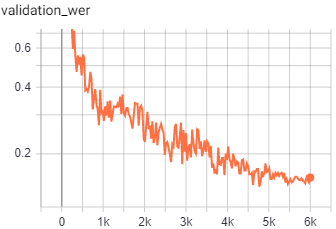
\includegraphics[width=100mm, keepaspectratio]{figures/an4_wer.png}
\caption{AN4 adatbázis validációs adathalmazán elért eredmények.}
\label{fig:TeXstudio}
\end{figure}

Arról, hogy a beállításaim tényleg megfelelőek a LibriSpeech 100 órás adathalmazán bizonyosodtam meg. Azért nem ezzel kezdtem, mert 100 órányi hanganyag tanítása jóval tovább tart, így minél kevesebbszer akartam végigfuttatni a tanítást az optimalizálás érdekében.

A LibriSpeech-hez egy nagyobb méretű architektúrát használtam. A mélyebb hálók jellemzően pontosabb eredményeket képesek elérni a paraméterszám növelése mellett. Összevetettem az eredeti, 5x1-es modellt a nagyobb, 12x1-es QuartzNet modellel és a korábban optimálisnak vélt epoch számmal és egy magasabb learning rate-el. A különbség az 5.2-es ábrán látható.

\begin{figure}[!ht]
\centering
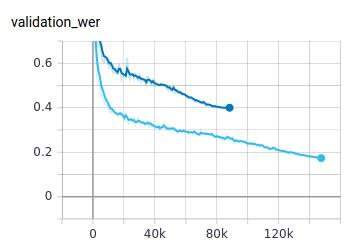
\includegraphics[width=100mm, keepaspectratio]{figures/architecture_comparrison.png}
\caption{LibriSpeech eredmények QuartzNet 5x1 (sötétkék) és 12x1 (világoskék) architektúrákon.}
\label{fig:TeXstudio}
\end{figure}

\section{Orosz nyelvű hálók}

Az orosz nyelvű implementációhoz már jó kiindulópontot jelentett a LibriSpeech-nél is alkalmazott architektúra. Az Mozilla Common Voice orosz adatbázisa átesett a szükséges formázásokon, és legeneráltam belőle a megfelelő .json fájlt. A legenerált fájlban odafigyeltem, hogy csak cirill betűk szerepeljenek, illetve szükség esetén kisbetűsítettem a szöveget.

\subsection{NeMo config fájl}

A NeMo a modellek leírásához config fájlokat használ. A fájlokban minden modellt és tanítást leíró paramétert meg lehet adni. Ezek közé tartozik a modell architektúrája, a használandó aktivációs rétegek, a learning rate és az epoch szám vagy az optimalizáló típusa.

Előnye, hogy könnyen módosítható és a programkódtól független. Megadhatók üresen hagyott paraméterek is, melyeket `???` el lehet jelölni. Ezeket később programkódból ki lehet tölteni, mint például a használandó manifest fájl elérési útját.

% kép?

\subsection{Szükséges módosítások}

A config fájlban két dolgot kellett átállítani az orosz nyelv használata előtt. Az egyik maguk a betűk, label-ek voltak, mivel az orosz ábécé merőben eltér az angolétól. A cirill karakterek könnyen kinyerhető a google translate orosz nyelvű virtuális billentyűzete segítségével.

A másik átállítandó paraméter a config fájl AudioToTextDataLayer részében a leiratok normalizálására szolgáló rész. Erre azért van szükség, mert alapból elvégezné a modell, de szeretnénk elkerülni, mivel angol nyelvre lett tervezve így egyéb nyelveken nem működne megfelelően. 

% cite https://github.com/NVIDIA/NeMo/issues/234

\subsection{Architektúrák}

A kísérletezéshez 2 különböző architektúrát, 12x1 és 15x5-et használtam. A választáson fő szempontja az volt, hogy ilyen architektúrákhoz rendelkeztem előre tanított angol nyelvű modellekkel. Ezeket később a transfer learning-nél használtam fel, és összehasonlítottam a véletlenszerűen inicializált súlyú modellek eredményeivel.

A tanításokat a Mozilla és Radio2 adatbázisán is futtattam. A Radio2-es adatbázis túl nagynak bizonyult, a hanganyagok méretét 8.7 másodpercben maximalizáltam, szemben a megszokott 16.7 másodperccel, így az összes tanítóadat 100 órát tett ki.

% 100 ÓRA HELYETT PONTOS ÉRTÉK!!!

Fontos kiemelni, hogy a tanítás közbeni pontosság teszteléséhez, azaz a validációhoz mindegyik esetben a Mozilla adatbázishoz tartozó tesztadatokat használtam. A pontosságot külön-külön megvizsgáltam a Radio2-es adatbázisból leválasztott, tanításhoz fel nem használt hanganyagokon is.

\subsection{Transfer learning}

A Transfer learning-hez előre betanított modelleket kellett szerezzek. A QuartzNet 15x5 architektúrájú modell könnyen elérhető volt, az Nvidia által szabad rendelkezésre volt bocsájtva. A 12x1-es architektúrát konzulensem Dr. Mihajlik Péter bocsájtott rendelkezésemre. Ez a modell kevesebb adaton és rövidebb ideig tanult mint a 15x5-ös, de jobb kiindulópont volt, aminek előállítására lehetőségem lett volna.

A modell betöltése hasonlóan történt a checkpoint-ból való folytatás betöltéséhez, azzal a különbséggel, hogy nem a teljese modellt használtam, csupán az encoder részét. Ez fontos különbség, hiszen a decoder használhatatlan lett volna, mivel az angol nyelvre lett tanítva. Így a decoder-hez véletlenszerűen inicializált súlyokat használtam, és a modell encoder részének súlyai kerültek átemelésre.

A tanítás ezen felül a megszokott szerint zajlott a megfelelő config fájl betöltésével, tanítóadatok és trainer beállításával, a súlyok kimentésével.
%----------------------------------------------------------------------------
\chapter{Összefoglalás}
%----------------------------------------------------------------------------

\begin{table}[ht]
	\footnotesize
	\centering
	\begin{tabular}{ p{2.5cm} p{2.5cm} p{1.5cm} p{1.5cm} p{1cm} p{1.5cm} p{1.5cm} }
		\toprule
		\textbf{Architektúra (QuartzNet)} & \textbf{Adathalmaz} & \textbf {Transfer Learning (I/N)} & \textbf{Tanítás hossza órában} & \textbf{Epoch szám} & \textbf{Training WER (\%)} & \textbf{Validation WER (\%)} \\
		\midrule
		5x1 & an4 & N & 0.25 & 200 & - & 15.65 \\
		\hline
		5x1 & LS100 & N & 9 & 100 & 31.23 & 40.04 \\
		\hline
		12x1 & LS100 & N & 14.25 & 100 & 19.92 & 25.65 \\
		\hline
		12x1 & orosz\_rövid & N & 8 & 200 & 10.5 & 58.4 \\
		\hline
		15x5 & orosz\_rövid & I & 11.5 & 100 & 8.84 & 41.95 \\
		\hline
		12x1 & orosz\_közepes & N & 18.5 & 200 & 7.26 & 42.56 \\
		\hline
		12x1 & orosz\_közepes & N & 8 & 100 & 14.53 & 56.3 \\
		\hline
		12x1 & orosz\_közepes & I & 9 & 100 & 19.42 & 52.01 \\
		\hline
		15x5 & orosz\_közepes & N & 35 & 100 & 10.79 & 45.6 \\
		\hline
		15x5 & orosz\_közepes & I & 36.5 & 100 & 5.63 & 30.89 \\
		\hline
		12x1 & orosz\_hosszú & I & 27 & 63 & 41.93 & 67.42 \\
		\hline
		15x5 & orosz\_hosszú & I & 45 & 33 & 31.91 & 59.25 \\
		\bottomrule
	\end{tabular}
	\caption{A kipróbált modellek, azok architektúrája és az általuk elért WER eredmények.}
\end{table}

Az összes modellnél a későbbi összehasonlíthatóság végett 0.01-es learning rate-et használtam 0.001-es weight decay-el, CosineAnnealing ütemezővel, melynek 100 bemelegítő lépés volt megadva.

\section{Különböző architektúrák összehasonlítása}

A nagyobb modellek pontosabb eredményeket és alacsonyabb WER-t értek el adatbázistól függetlenül. Viszont ez az idő drasztikus növekedésével járt együtt. A 12x1-es architektúra nagyjából 5 millió paramétert, míg a 15x5-ös architektúra 18.9 millió paramétert használt. Futtatási idő esetén ez azt eredményezte, hogy fele annyi epoch-hoz másfélszer annyi időre volt szüksége, ami 3-szoros sebesség csökkenést eredményez. Következtetésképp lehetőség szerint érdemes minél több erőforrással dolgozni, az idő csökkentése végett és a mélyebb háló útján elindulni a precízebb végeredmény céljából.

\begin{figure}[!ht]
\centering
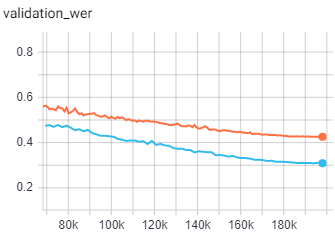
\includegraphics[width=100mm, keepaspectratio]{figures/architecture_12x1_vs_15x5.png}
\caption{15x5-ös - kék és 12x1-es - narancs architektúrák. Merőleges tengelyen a lépések, batchek száma, függőleges tengelyen a WER értéke.}
\end{figure}

A 6.1-es ábrán látható viszont a mélyebb, összetettebb háló előnye, hiszen ekvseebb epoch alatt pontosabb eredményeket, alacsonyabb validation WER értéket sikerült elérni vele, mint a 12x1 architektúrával.

\section{Véletlenszerűen inicializált vs transfer learning}

Minden esetben megállapítható, hogy a transfer learning nagyban javította az elért eredményeket, annak ellenére, hogy az átvett modell súlyai egy másik ábécével, másik nyelven lettek tanítva.  Látható, hogy az emberek által generált hangok, a nyelvek struktúrája és logikája erősen összefügg.

Látható, hogy a transfer learning-et a beszédfelismerés területén lehetőség szerint érdemes használni, hiszen lényegesen javíthatók vele a felismerési eredmények. Hátránya, hogy rendelkezni kell az előre tanított súlyokkal a megfelelő architektúrákhoz.

\begin{figure}[!ht]
\centering
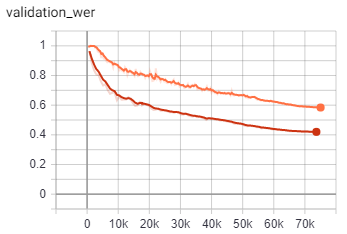
\includegraphics[width=100mm, keepaspectratio]{figures/12x1_pretrained_vs_random.png}
\caption{12x1-es architektúrák validation WER étékei pretrained - vörös és random inicializált - narancs színű súlyokkal. Merőleges tengelyen a lépések, batchek száma, függőleges tengelyen a WER értéke.}
\end{figure}

\section{Mozilla Common Voice és Radio2}

A két adatbázis fő különbsége az adatok mennyisége volt. A Radio2-ből nagyjából 200 órányi adatot használtam fel (orosz\_hosszú), míg a Mozilla Common Voice-ból 45 órányit (orosz\_közepes). Emiatt a Radio2-vel hosszabb tanításokra, de jobb általános eredményekre lehetett számítani.

Ennek megfigyelésére a két különböző adatbázison tanított modellek teljesítményét kell megvizsgálni. A orosz\_közepes tanított modell \~29\%-al jobb WER eredményt ért el az orosz\_hosszú adathalmazon tanított modellnél az orosz\_közepes-hoz tartozó teszt adathalamzon. Viszont az orosz\_hosszú-ból leválasztott teszt adathalmazon lényegesebb, \~37\% körüli érték volt az eltérés az orosz\_hosszú adathalmazon tanult adatok javára. Látható, hogy a nagyobb adatmennyiség egy általánosabban jobban teljesítő modellt eredményezett.

\section{Javítási lehetőségek}

A jobb WER eredmények végett alkalmazhatóak a neurális hálók esetén a gyakran használt augmentációs módszerek. Ezek az elérhető hanganyag mennyiséget dúsítják fel különböző módszerekkel. Ez lehet az eredeti hanganyag torzítása, levágása, zaj hozzáadása vagy sebességének módosítása.

Fontos különbség a megszokott neurális háló alapú beszédfelismerő rendszerekhez képest, hogy nem használtam az implementációmban nyelvmodellt, illetve a legegyszerűbb, greedy, dekódolási eljárással dekódoltam a kimeneti mátrixomat, ami szuboptimális eredményeket nyújt, hiszen ennél összetettebb módszerek szinte kizárólag jobb eredményekhez vezetnek\cite{decoder}. Ettől eltérő dekóder használata javíthat az eredményeken.

Nagyobb adatbázisok alkalmazása jobb általánosítást eredményez, ami a validációs WER érték csökkenésével jár együtt. Érdemes a különböző adatbázisokat összefogni és akár több ezer órányi adaton tanítani.

A sebesség növeléséhez a NeMo toolkit több lehetőséget is kínál. Az egyik a Mixed Precision\footnote{Mixed Precision lehetőség magyarázat az NVIDIA oldalán: \url{https://docs.nvidia.com/deeplearning/nemo/neural_mod_bp_guide/index.html}}, a másik módszer több GPU bevonása a tanítási folyamatba. Utóbbi esetben több, előre meghatározott GPU közt osztódik el az adat és kerül gyorsabb kiértékelésre.

Lehetséges még a tanítóadat pontos behatárolása. Mivel tanítás közben, a tanítási batch-ekbe különböző hosszúságú hangfájlok kerülnek betöltésre, így például egy 16-os batch méret esetén a GPU hamar kiértékeli az 5 másodperc hosszú hangfájlokat, de nem tud tovább haladni, míg a leghosszabbat, például egy 14 másodperceset nem értékelt ki. Ezen probléma elkerülése, és a GPU jobb kihasználása végett célszerű nagyjából egyforma hosszúságú adatokat felhasználni a tanításhoz.

Természetesen javulást eredményezhet a hiperparaméterekkel való kísérletezés, azok finomítása. Különböző adatok, nyelvek vagy architektúrák más-más paraméterekkel működnek jobban, nincsenek bevett számok, legfeljebb megközelítőleg.

\section{Végső gondolatok}

A beszédfelismerés már régóta velünk van, de egyre inkább elterjed és bekerül a köztudatba, mindennapjainkba a pontosság növekedésének következtében. Ehhez nagyban hozzájárul a klasszikus HMM-től eltérő, napjainkban egyre inkább felkapott megközelítés a mély neuron háló alapú, end-to-end beszédfelismerés. Egyre több toolkit, és platform jelenik meg, amelyek könnyítik a neurális hálókkal való munkát, azok fejlesztését.

Az angoltól eltérő nyelvű automatikus beszédfelismerő rendszerek fejlesztése és kutatása fontos terület, hiszen a különböző nemzetek polgárai a saját nyelvükön akarnak beszélni. Segítséget nyújthatnak ebben a folyamatban a precíz, angol nyelvű modellek a transfer learning által, aminek következtében drasztikus javulás érhető el az új modell WER pontosságánál.

A nap mint nap megjelenő újabb architektúrák implementálásával a pontosság tovább növelhető, így korábban elképzelhetetlen, az embernél is nagyobb pontosságú beszédfelismerés valósítható meg, mely az élet számos területén használható fel.
% Acknowledgements
%~~~~~~~~~~~~~~~~~~~~~~~~~~~~~~~~~~~~~~~~~~~~~~~~~~~~~~~~~~~~~~~~~~~~~~~~~~~~~~~~~~~~~~
%----------------------------------------------------------------------------
\chapter*{\koszonetnyilvanitas}\addcontentsline{toc}{chapter}{\koszonetnyilvanitas}
%----------------------------------------------------------------------------

Köszönöm az útmutatást, javaslatokat és minden egyéb segítéget a szakdolgozatom elkészítéséhez konzulensemnek,  Dr. Mihajlik Péternek.


% List of Figures, Tables
%~~~~~~~~~~~~~~~~~~~~~~~~~~~~~~~~~~~~~~~~~~~~~~~~~~~~~~~~~~~~~~~~~~~~~~~~~~~~~~~~~~~~~~
%\listoffigures\addcontentsline{toc}{chapter}{\listfigurename}
%\listoftables\addcontentsline{toc}{chapter}{\listtablename}


% Bibliography
%~~~~~~~~~~~~~~~~~~~~~~~~~~~~~~~~~~~~~~~~~~~~~~~~~~~~~~~~~~~~~~~~~~~~~~~~~~~~~~~~~~~~~~
\addcontentsline{toc}{chapter}{\bibname}
\bibliography{bib/mybib}


% Appendix
%~~~~~~~~~~~~~~~~~~~~~~~~~~~~~~~~~~~~~~~~~~~~~~~~~~~~~~~~~~~~~~~~~~~~~~~~~~~~~~~~~~~~~~
% %----------------------------------------------------------------------------
\appendix
%----------------------------------------------------------------------------
\chapter*{\fuggelek}\addcontentsline{toc}{chapter}{\fuggelek}
\setcounter{chapter}{\appendixnumber}
%\setcounter{equation}{0} % a fofejezet-szamlalo az angol ABC 6. betuje (F) lesz
\numberwithin{equation}{section}
\numberwithin{figure}{section}
\numberwithin{lstlisting}{section}
%\numberwithin{tabular}{section}

%----------------------------------------------------------------------------
\section{A TeXstudio felülete}
%----------------------------------------------------------------------------
\begin{figure}[!ht]
\centering
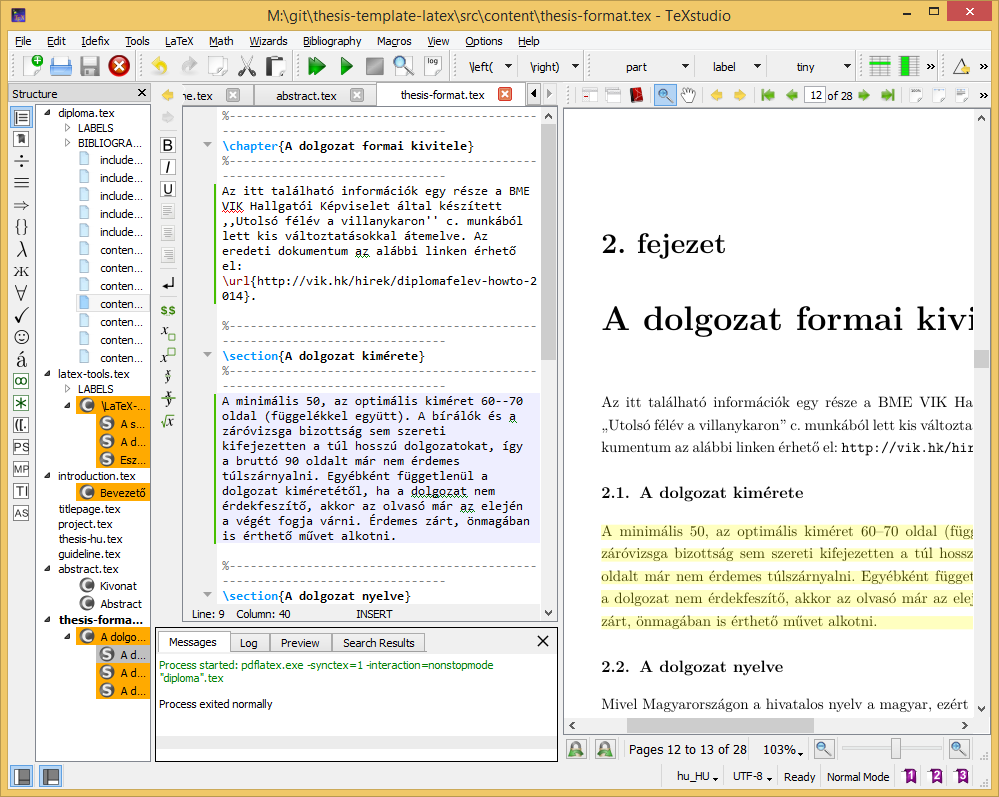
\includegraphics[width=150mm, keepaspectratio]{figures/TeXstudio.png}
\caption{A TeXstudio \LaTeX-szerkesztő.} 
\end{figure}

%----------------------------------------------------------------------------
\clearpage\section{Válasz az ,,Élet, a világmindenség, meg minden'' kérdésére}
%----------------------------------------------------------------------------
A Pitagorasz-tételből levezetve
\begin{align}
c^2=a^2+b^2=42.
\end{align}
A Faraday-indukciós törvényből levezetve
\begin{align}
\rot E=-\frac{dB}{dt}\hspace{1cm}\longrightarrow \hspace{1cm}
U_i=\oint\limits_\mathbf{L}{\mathbf{E}\mathbf{dl}}=-\frac{d}{dt}\int\limits_A{\mathbf{B}\mathbf{da}}=42.
\end{align}


%\label{page:last}
\end{document}
